%% Chapter 11 — LLM Serving
\setcounter{chapter}{10}
\chapter{LLM Serving}
\chaptersubtitle{Autoregression, the KV cache, continuous batching — and the operating system that moved inside the engine}

\begin{calloutbox}{tbbblue}{tbbbluefill}
{\normalsize\bfseries\color{tbbblue}Learning objectives}\par\vspace{3pt}
\begin{tbbitemize}
  \item Explain why request-level latency SLOs go meaningless for generative traffic, and rewrite them with the \textbf{two clocks} — TTFT and TPOT — budgeted by two human constants (Miller 1968; reading speed).
  \item Dissect one generation into \textbf{prefill and decode}, compute each phase's arithmetic intensity, and predict from Chapter 10's roofline which resource each phase exhausts.
  \item Derive the \textbf{KV cache} from what attention re-reads, size it from the model card, and budget VRAM into weights, runtime, and a cache pool — making concurrency a memory number.
  \item Explain \textbf{continuous batching} (iteration-level scheduling) as the repair of Chapter 9's broken assumption, including prefill–decode interference and chunked prefill.
  \item Explain \textbf{PagedAttention} as virtual memory transplanted into attention — block tables, sharing, copy-on-write — and why reclaimed waste was worth 2–4× measured throughput.
  \item Operate \textbf{vLLM}: map it onto Chapter 9's six organs, read its metrics, serve a quantized (AWQ) model, and measure TTFT/TPOT honestly under concurrency — the lab, and the project's new SLO sentence.
\end{tbbitemize}
\end{calloutbox}

\vspace{2.5pt}

\begin{calloutbox}{tbbteal}{tbbtealfill}
{\normalsize\bfseries\color{tbbteal}Key terms}\par\vspace{3pt}
autoregressive generation · prefill vs. decode · TTFT · TPOT / tokens-per-second · streaming (SSE) · reading-speed floor · KV cache · GQA / MQA · KV budget · admission \& preemption · continuous batching · iteration-level scheduling (Orca) · prefill–decode interference · chunked prefill · PagedAttention · block table · prefix caching · copy-on-write · vLLM · speculative decoding · token-aware load testing
\end{calloutbox}

\vspace{2.5pt}

\begin{calloutbox}{tbblightgray}{tbbboxfill}
{\normalsize\bfseries\color{tbbink}Chapter outline}\par\vspace{3pt}
\textbf{11.1} The model talks back — and the dashboard lies    \textbf{11.2} Anatomy of a generation: two phases, two clocks    \textbf{11.3} The KV cache: memory is the new concurrency    \textbf{11.4} Continuous batching: the city bus    \textbf{11.5} PagedAttention and vLLM: the OS moves inside    \textbf{11.6} Lab: serve, stream, and measure a real LLM — followed by a summary, exercises, and further reading.
\end{calloutbox}

\section{The Model Talks Back — and the Dashboard Lies}

Every serving system this course has built shares one silent assumption: \textbf{a request is a unit of work}. A classify call costs one forward pass; the pass takes milliseconds; you promise a percentile of that number and provision for it. Chapters 7 through 10 measured, optimized, and priced that world — and last week ended in triumph: the 3B chat model, TensorRT-INT8-optimized, held its p99 under 500 ms at 57 req/s per L4, and the fleet bill halved, as promised. This Monday, the beta users arrived. They did not send the sweep's canned prompts. They asked for cover letters:

\begin{terminalbox}
\begin{Verbatim}[breaklines=true,breakanywhere=true,fontsize=\small,formatcom=\color{tbbtermfg},codes=\tbbcodeactive]
# monday 09:12. the Week-10 stack (INT8, 4 x L4), meeting REAL
# chat traffic for the first time. locust replays the beta logs:
$ locust -f chat_replay.py --headless -u 32 -r 4 --run-time 10m
 Type  Name     # reqs   # fails |  Avg     p50      p99   | req/s
 POST  /chat     4,102   0(0.0%) | 3,846   2,910   11,400  |  6.8
# p99 = 11.4 SECONDS against a 500 ms SLO. dashboard: solid red.
$ kubectl top pod -l app=chat      # surely something is dying?
NAME         CPU(cores)   MEMORY
chat-7f9b4   3210m        11.2Gi   # ...healthy.
$ nvidia-smi --query-gpu=utilization.gpu --format=csv,noheader
94 %                                # busy AND healthy.
# nothing is broken. the ANSWERS got long:
#   "reset my password?"        ->  40 tokens,   0.9 s
#   "write my cover letter..."  -> 700 tokens,  14.8 s
# the request stopped being a unit of work. the SLO measures noise.
\end{Verbatim}
\end{terminalbox}
\figcaption{Exhibit 11-A  The p99 explosion. Every component passes its health check; the SLO is violated by a factor of 20; and the culprit is not a bug but a distribution — response length now varies 100×, and request latency inherits all of it. The metric died, not the system.}

Sit with the exhibit's strangeness for a moment, because it is a new \textit{kind} of failure for this course. In Chapter 7's vocabulary, nothing regressed: the machine does the same work per token it did on Friday. What broke is the \textbf{contract's unit}. A "request" now spans three orders of magnitude of work — 40 tokens to 4,000 — decided not by your capacity planning but by \textit{what the user asks and how the model chooses to answer}. Promising a request-level p99 over that distribution is promising the weather. And no amount of Chapter 10 optimization fixes it: halve the per-token cost and the cover letter still takes seven seconds. The mean describes nobody — and now the p99 doesn't either, because it tracks answer length, not system health.

\subsection*{The oldest interface in computing, rediscovered}

The way out was discovered twice, fifty-five years apart. This course opened Week 2 with time-sharing — CP-67 carving one mainframe into many — but the detail that matters now is \textit{what the terminal did}: it \textbf{typed back}. A teletype at 10 characters per second delivered a computer's answer as a stream, and users, it turned out, loved it — the machine felt alive, engaged, \textit{working for them}. In 1968, IBM's Robert Miller measured the psychology under that feeling and produced three numbers that have survived every interface revolution since: below \textbf{0.1 s} an action feels instantaneous; up to \textbf{1 s} thought flows uninterrupted; past \textbf{10 s} attention collapses and the user task-switches. Add one more human constant — people read at roughly 250 words per minute, or 5–7 tokens per second — and the entire design space of conversational AI is already drawn, in 1968, on paper.

Now re-read Exhibit 11-A against those constants. The un-streamed cover letter lands at 14.8 s — deep in Miller's abandonment zone. But the model \textit{produced its first word} within a few hundred milliseconds and the rest at \textasciitilde{}50 tokens/second, seven times faster than anyone reads. Delivered as a stream, the identical computation sits \textit{comfortably inside} the 1-second flow zone and stays ahead of the reader forever after. \textbf{Streaming does not make the answer faster; it changes which clock the user experiences.} That is the actual innovation ChatGPT shipped to a hundred million people — not a latency optimization but a contract renegotiation, and the reason every chat product since types its answers like a 1968 teletype. (§7.2 named this mode and promised its clocks would get SLOs "in Week 11." It is Week 11.)

\begin{tbbfigure}
  \adjustbox{max width=0.94\linewidth,max totalheight=0.46\textheight}{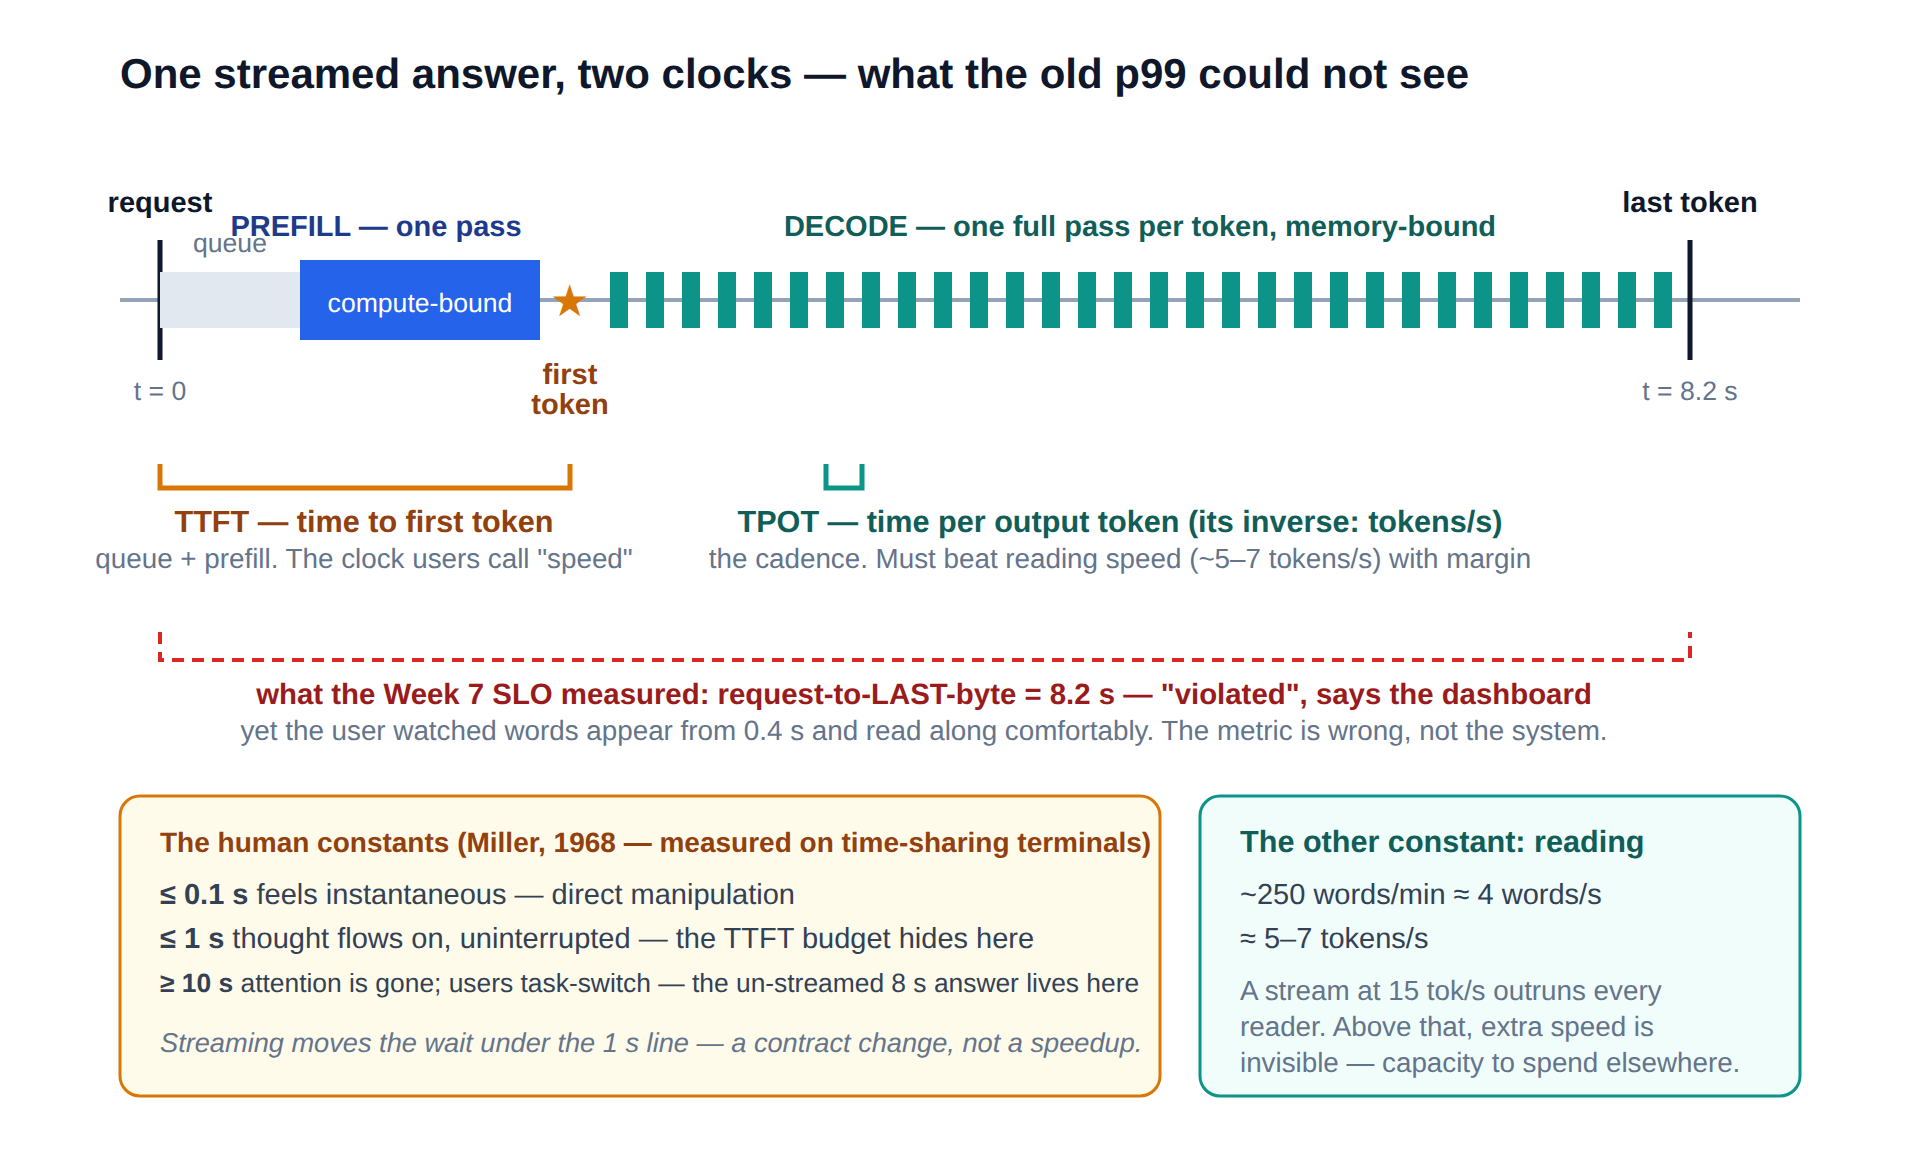
\includegraphics{figures/fig11-1_twoclocks.png}}\\[3pt]
  \figcaption{Figure 11-1  One streamed answer, two clocks. TTFT (queue + prefill) answers "is it responsive?"; TPOT answers "does it outrun my reading?"; and the old request-to-last-byte p99 answers a question nobody asked. Miller's 1968 thresholds and reading speed are the budgets.}
\end{tbbfigure}

So the project's SLO sentence gets rewritten, not discarded — and the rewrite is kinder than you might fear. The old promise ("p99 ≤ 500 ms") was, without knowing it, a promise about \textit{responsiveness} — it survives intact as the \textbf{TTFT budget}, because 500 ms sits nicely under Miller's 1-second line. What gets added is a \textbf{cadence clause} (per-stream tokens/second, floored comfortably above reading speed) and a \textbf{capacity restatement}: not requests per second — meaningless across a 100× length spread — but \textit{concurrent streams}. The full sentence, which the lab will teach you to measure: \textbf{"TTFT p99 ≤ 500 ms; per-stream ≥ 15 tokens/s p50; at 100 concurrent streams on the 4-replica L4 fleet, within \$900/month."} Every clause of Chapter 7's discipline — percentile, threshold, load, price — survives; only the units changed species.

\subsection*{The second exhibit: something is remembering}

The same afternoon delivers this chapter's other mystery. A teammate runs the multi-turn demo for the class — and keeps one eye on \code{nvidia-smi}, a habit Chapter 2 installed. The model is 6 GB. Watch:

\begin{terminalbox}
\begin{Verbatim}[breaklines=true,breakanywhere=true,fontsize=\small,formatcom=\color{tbbtermfg},codes=\tbbcodeactive]
# 14:00, demo day. multi-turn chat, ~30 slow-growing conversations.
$ watch -n 60 nvidia-smi --query-gpu=memory.used --format=csv,noheader
14:00    9,812 MiB    # weights (6 GB) + runtime + a few young chats
14:07   14,203 MiB    # ...the demo continues, nothing new deployed...
14:15   19,540 MiB    # no bigger model. no leak. no new users.
14:21   22,911 MiB    # the server is REMEMBERING something.
14:22   torch.cuda.OutOfMemoryError: CUDA out of memory. Tried to
        allocate 448.00 MiB (GPU 0; 23.99 GiB total capacity)
# exit 137's GPU cousin (Chs. 3/5) - and note the amount it wanted:
# 448 MiB. remember that number. §11.3 will compute it from scratch.
\end{Verbatim}
\end{terminalbox}
\figcaption{Exhibit 11-B  The creep. Memory grows with every token of every conversation while weights stay constant — then the allocator asks for exactly 448 MiB more and dies. Nothing leaked. The model keeps a growing notebook about every open conversation, and nobody budgeted for the notebook.}

Two exhibits, two mysteries, one chapter. Exhibit A says the \textit{time} axis broke: latency must be re-contracted per token. Exhibit B says the \textit{memory} axis broke: something grows per token, and it — not compute — decides how many users fit on a GPU. Both trace to a single mechanical fact you can hold in one sentence: \textbf{a language model answers by running its entire forward pass once per output token, consulting everything it has produced so far.} That loop is §11.2. The notebook it consults is §11.3 (and 448 MiB will turn out to be one 4,096-token conversation's notebook, to the megabyte). The scheduler that keeps a GPU full of such loops is §11.4, the memory manager that stops wasting the notebook's shelf space is §11.5 — and the lab, §11.6, puts you in front of all of it with vLLM, a stopwatch, and ten dollars of T4 time.

One promise about the promises: this chapter is where more of the course's IOUs come due than anywhere else. Chapter 1 called the KV cache "the star of Week 11" and Kwon et al. "required reading." Chapter 6 owes you the sticky-session verdict and the stream that dies at exactly 60.0 seconds. Chapter 7 owes streaming its SLOs. Chapter 9's Box 9-1 fine print — \textit{requests must be similar-shaped} — detonates here, and its Further Reading pointed at Orca "after the KV cache lecture." Chapter 10 owes you the per-group INT4 vocabulary in action, the speculative-decoding lever, and an answer to the matvec whose AI ≈ 1. All of it pays out below.

\begin{calloutbox}{tbbpurple}{tbbpurplefill}
{\normalsize\bfseries\color{tbbpurple}Think About It}\par\vspace{3pt}
\begin{tbbitemize}
  \item Exhibit 11-A's service is "healthy by every dashboard" yet failing its SLO by 20×. Name three dashboards from Chapters 5–9 that would all show green here, and the ONE number (not yet on any dashboard) that actually predicts user anger. Where does that number come from mechanically?
  \item Miller's thresholds were measured on 1968 time-sharing terminals; reading speed is older still. Argue for or against: "conversational AI product design is over-determined by constants that predate it by half a century." What, if anything, about LLMs adds a genuinely NEW constant?
  \item A PM proposes fixing Exhibit 11-A by capping max\_tokens at 100 ("no more cover letters"). Using the serving triangle and the two clocks, enumerate what this trades away, which users notice, and why streaming is the strictly kinder cut of the same cake.
  \item Exhibit 11-B's allocator died asking for 448 MiB. Without reading ahead: list every quantity from Chapters 1–10 you would need to predict that number from a model card, and take a guess at what grows. (§11.3 grades your guess.)
\end{tbbitemize}
\end{calloutbox}

\section{Anatomy of a Generation: Two Phases, Two Clocks}

Strip the mystery first. A transformer language model is a function that reads a token sequence and outputs \textbf{one probability distribution over the next token}. That is all it can do. To produce a 200-token answer, the serving stack must therefore run the model 200 times: feed the prompt, sample token \#1; append it, run again, sample token \#2; append, run, sample — a loop, called \textbf{autoregressive generation}, that ends only when the model emits a stop token or hits a limit. Everything strange about LLM serving — the two clocks, the growing memory, the broken batcher, the exotic engines — falls out of this one loop and the roofline you already own. So let us take one request apart with Chapter 10's instruments.

\begin{tbbfigure}
  \adjustbox{max width=0.94\linewidth,max totalheight=0.46\textheight}{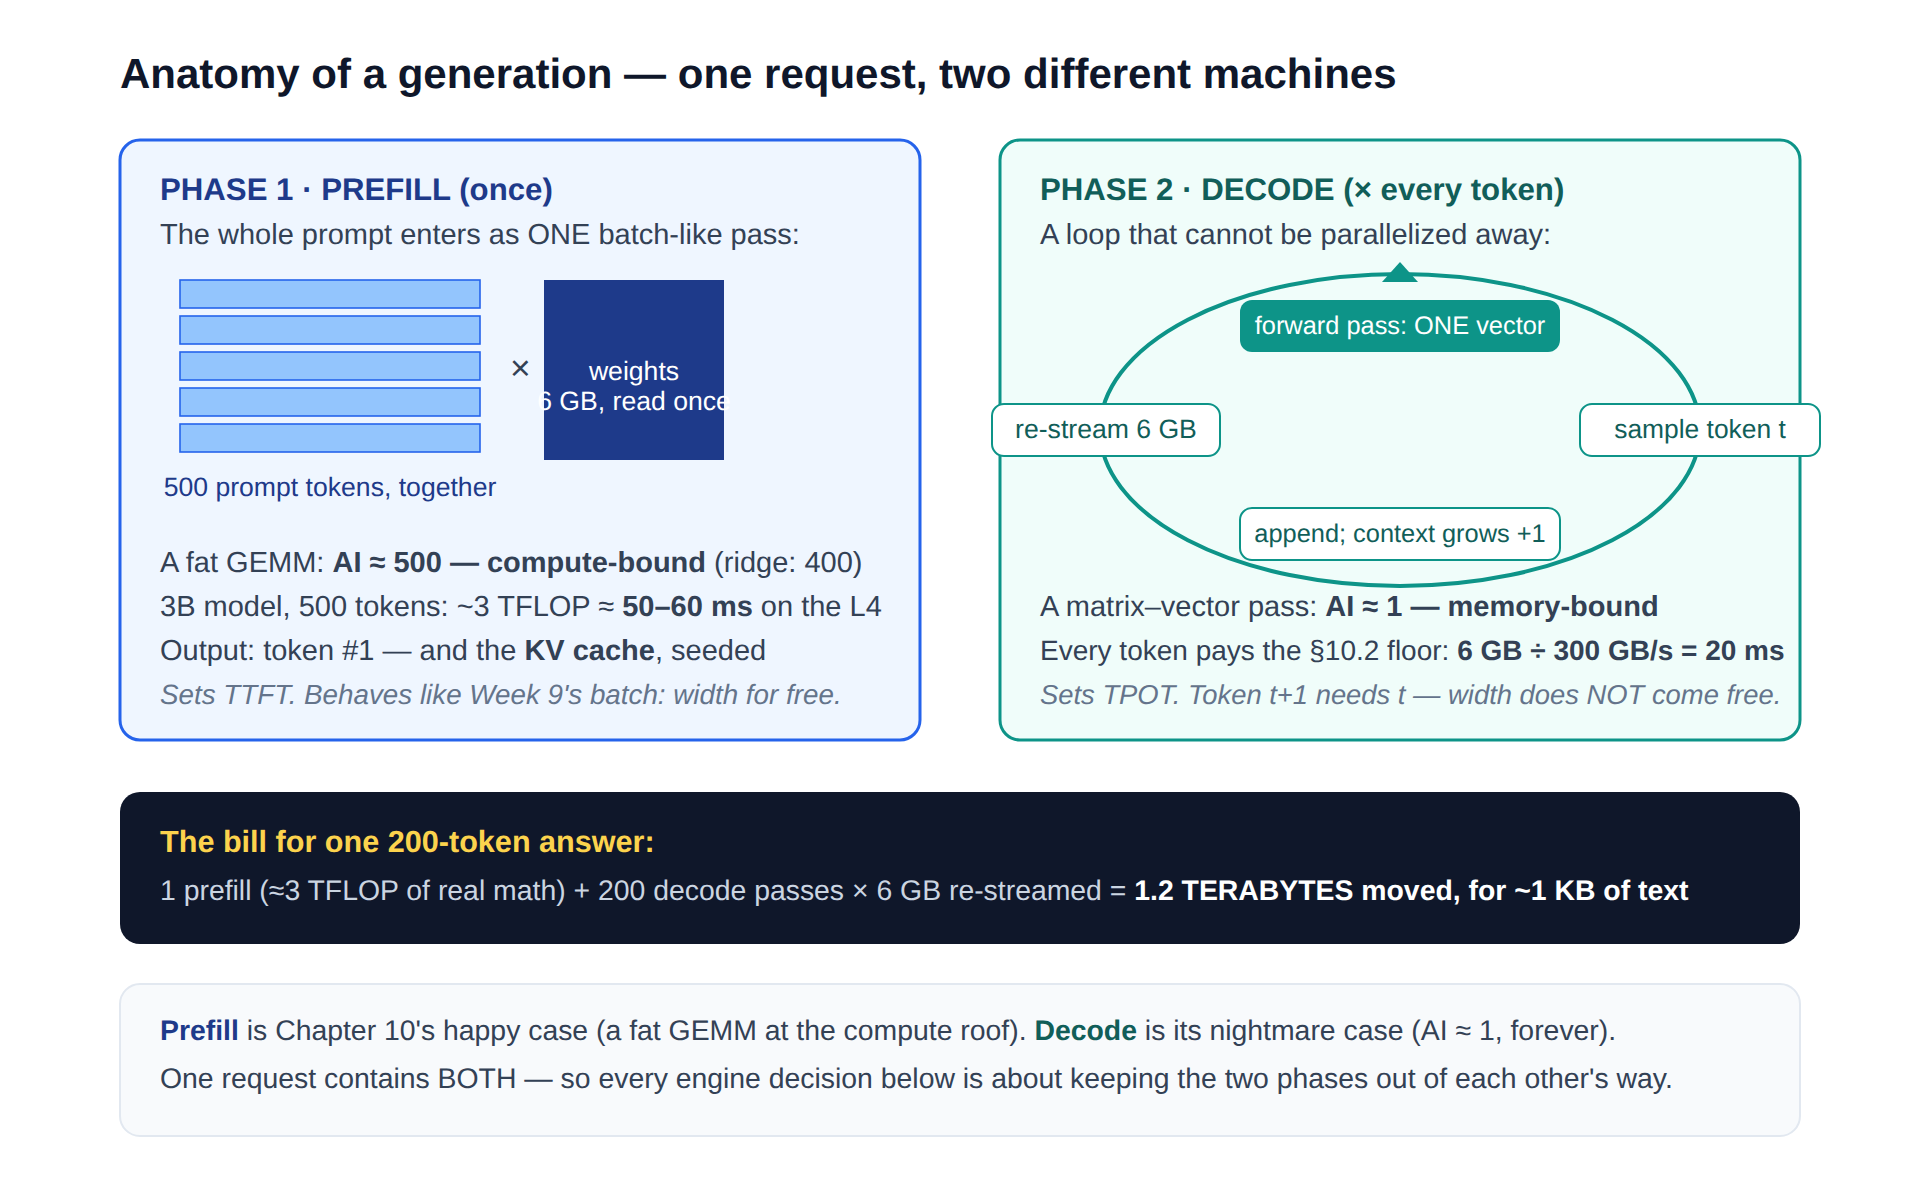
\includegraphics{figures/fig11-2_autoregress.png}}\\[3pt]
  \figcaption{Figure 11-2  One request, two machines. Prefill devours the whole prompt in a single compute-bound pass and seeds the cache; decode then loops — one full forward pass per token, re-streaming every weight, memory-bound forever. The engine's whole job is keeping these two phases out of each other's way.}
\end{tbbfigure}

\subsection*{Prefill: the fat GEMM you already know}

The first pass is special. The prompt's tokens are all \textit{known} — nothing must be sampled between them — so the model processes all 500 of them \textbf{together, in one pass}, exactly like a Week 9 batch of 500 items that happen to attend to each other. Chapter 10's trio told you what that is: a fat GEMM. Arithmetic intensity ≈ the token count (each streamed weight does 500 tokens' worth of work), so at 500 tokens the pass sits \textit{above} the L4's ridge of \textasciitilde{}400 — genuinely \textbf{compute-bound}, the roofline's happy corner. The cost is honest work: \textasciitilde{}2 FLOPs per parameter per token × 3B × 500 ≈ \textbf{3 TFLOP}, which the L4 grinds through in 50–60 ms at realistic efficiency. Prefill produces two things: the \textbf{first output token} — so prefill time is almost all of TTFT — and a by-product whose name you have been waiting two exhibits for: the K and V tensors of every prompt token, cached for the loop to come (§11.3).

\subsection*{Decode: the matvec that never ends}

Then the loop begins, and the machine changes species. Each decode step feeds \textbf{one token} — the one just sampled — through the full network to get the next distribution. One token means matrix–\textit{vector} work throughout: Chapter 10's opening workload, AI ≈ 1, the byte-delivery service with math attached. Every step must re-stream all 6 GB of weights to perform \textasciitilde{}6 GFLOP, so every step pays the §10.2 floor: \textbf{6 GB ÷ 300 GB/s = 20 ms}, with a millisecond or two of launches and sampling on top. And the steps cannot overlap \textit{within a sequence}: token t+1's input \textbf{is} token t, so the loop is inherently serial — no batching, no compiler, no cleverness removes that dependency (only §11.5's speculative decoding even bends it). Decode sets TPOT; TPOT is pinned to the memory wall; and that is why Chapter 10 kept calling batch-1 generation "the wall at its cruelest."

\begin{terminalbox}
\begin{Verbatim}[breaklines=true,breakanywhere=true,fontsize=\small,formatcom=\color{tbbtermfg},codes=\tbbcodeactive]
# one instrumented request against a single unloaded L4 replica:
$ python two_clocks.py --url http://chat-l4:8000 --prompt 500tok.txt
tokenize + queue + prefill (500 tok):     73.8 ms   <- TTFT
decode: 200 tokens in 4.28 s:             21.5 ms/token  (46.5 tok/s)

# sanity, against §10.2 (no profiler, as always):
#   decode floor: 6 GB / 300 GB/s        = 20.0 ms  -> observed 21.5
#   overhead: launches+sampling+attention =  1.5 ms  -> a small a
#   prefill: 3 TFLOP / (~55 TFLOPS eff.) = ~55 ms   -> observed ~65
# prefill did 500 tokens of work in ~3.4 decode-tokens' time.
# two machines, one API. every engine decision follows from this.
\end{Verbatim}
\end{terminalbox}
\figcaption{Transcript 11-1  The two clocks, measured and reconciled with Chapter 10's floors. Prefill is compute (500 tokens for the price of \textasciitilde{}3.4 decode steps); decode is bandwidth (the 20 ms floor, plus small change). TTFT ≈ queue + prefill; TPOT ≈ the floor.}

\subsection*{The clocks get their SLOs — and Little's law returns for streams}

Now the §11.1 contract can be engineered instead of merely declared. \textbf{TTFT} is queue + tokenize + prefill: its floor is prefill compute (\textasciitilde{}65 ms for a 500-token prompt), so the 500 ms budget leaves \textasciitilde{}430 ms for queueing — a real budget, spendable on batching admission (§11.4), and the reason TTFT, not TPOT, is what load kills first. \textbf{TPOT} is the decode floor plus whatever the scheduler adds: 21.5 ms unloaded (46 tok/s), degrading gracefully as concurrency shares the bandwidth (§11.3 computes exactly how). \textbf{End-to-end} still exists — a 200-token answer lands at 73.8 ms + 199 × 21.5 ms ≈ \textbf{4.4 s} — but it is now a \textit{derived} quantity, dominated by answer length, reported but not promised. And note what the stream buys: the reader consumes those 200 tokens over \textasciitilde{}30 seconds; the system delivered them in 4.4 — the stream runs seven times ahead of the eye it feeds.

Capacity planning also survives — via a souvenir. Chapter 7's \textbf{L = λW} does not care what a "customer" is, so redefine one: a \textit{stream} occupies a seat for W ≈ TTFT + N·TPOT seconds. At 200-token answers, W ≈ 4.4 s — so a replica holding 32 concurrent streams (§11.3 explains where 32 comes from) can absorb λ = 32 ÷ 4.4 ≈ \textbf{7.3 requests/s} in steady state. Check that against Exhibit 11-A: the failing fleet was measured at 6.8 req/s with utilization pinned — the law, holding to within noise, on the day everything "broke." The formula that sized Chapter 2's fleet sizes this one; only W changed meaning.

\begin{calloutbox}{tbbpurple}{tbbpurplefill}
{\normalsize\bfseries\color{tbbpurple}Think About It}\par\vspace{3pt}
\begin{tbbitemize}
  \item Transcript 11-1's prefill did 500 tokens of work in the time of 3.4 decode tokens. Compute the effective FLOPs utilization of each phase against the L4's 121 TFLOPS, and state — in roofline vocabulary — where the other \textasciitilde{}97\% of decode's compute capacity went.
  \item A teammate proposes "speed up TTFT by shortening prompts" vs. another's "speed up TTFT by admitting prefills ahead of decodes." Which clock does each proposal tax, for whom, and what §11.4 mechanism formalizes the second?
  \item Recompute Transcript 11-1 for the INT8 variant Chapter 10 shipped (3 GB weights, same GPU). Which clock improves, by how much, and why does the OTHER clock barely move? (Hint: prefill is compute-bound.)
  \item Use L = λW to size the WHOLE fleet: 100 concurrent streams required, W ≈ 4.4 s. What arrival rate can the product sustain? Now double average answer length. Which of the three SLO clauses breaks first, and what would you buy to fix it?
\end{tbbitemize}
\end{calloutbox}

\section{The KV Cache: Memory Is the New Concurrency}

Exhibit 11-B's server was "remembering something," and here it is. Inside every transformer layer, attention lets the current token consult every previous token — mechanically, it compares the current token's \textit{query} vector against each past token's \textbf{key} vector and blends their \textbf{value} vectors. Those K and V vectors are deterministic functions of each token (once it is fixed in place), which exposes a choice. \textbf{Recompute} them every step, and step t must push all t−1 previous tokens through every layer again just to re-derive what was already known — by mid-conversation each new token costs a prefill, and a 2,000-token chat performs on the order of two \textit{million} redundant token-layer computations. \textbf{Or cache them}: compute each token's K and V exactly once, store them, and let every later step read them from VRAM. Every serving stack on earth chooses the cache. The loop's compute stays flat per token — and the memory grows by one K,V row per layer, per token, for as long as the conversation lives. That growth is the creep.

\subsection*{Size it from the model card — no folklore required}

The per-token cost reads straight off the architecture. The course's 3B model has 28 layers and — like nearly every modern LLM — \textbf{grouped-query attention (GQA)}: its 24 query heads \textit{share} 8 KV heads of 128 dimensions each, precisely so that this cache (not the compute) shrinks 3×. Per token, per layer, it stores one K and one V vector of 8 × 128 values; in FP16 that is 2 × 28 × 8 × 128 × 2 bytes = \textbf{114,688 bytes ≈ 112 KB per token}. A 4,096-token conversation therefore holds 4,096 × 114,688 bytes = \textbf{469,762,048 bytes = 448.00 MiB} — to the byte, the allocation Exhibit 11-B died requesting. The mystery was never a leak; it was thirty conversations each carrying up to half a gigabyte of perfectly legitimate memory that nobody had budgeted, growing one 112 KB row at a time.

\begin{terminalbox}
\begin{Verbatim}[breaklines=true,breakanywhere=true,fontsize=\small,formatcom=\color{tbbtermfg},codes=\tbbcodeactive]
$ python kv_math.py --layers 28 --kv-heads 8 --head-dim 128 --dtype fp16
per token:            2 x 28 x 8 x 128 x 2 B = 114,688 B  (112 KB)
per 4k conversation:  4096 x 112 KB           = 448.00 MiB   # !!

# now budget the L4 (24 GB), vLLM-style at 90% utilization:
  usable            24.0 x 0.90 = 21.6 GB
  weights (FP16)                -  6.0 GB   # resident forever
  activations + CUDA + runtime  -  2.5 GB
  KV pool                       = 13.1 GB  -> ~115,000 tokens
# = 28 conversations at 4k. or 115 at 1k. THAT is your concurrency.
# note what is NOT in this arithmetic: FLOPS. compute stopped being
# the binding resource the moment the model started talking back.
\end{Verbatim}
\end{terminalbox}
\figcaption{Transcript 11-2  The cache, sized from the model card — and Exhibit 11-B's 448 MiB derived rather than observed. The L4's seat count is a division problem: 13 GB of pool over 112 KB per token. Concurrency became a memory number.}

\begin{tbbfigure}
  \adjustbox{max width=0.94\linewidth,max totalheight=0.46\textheight}{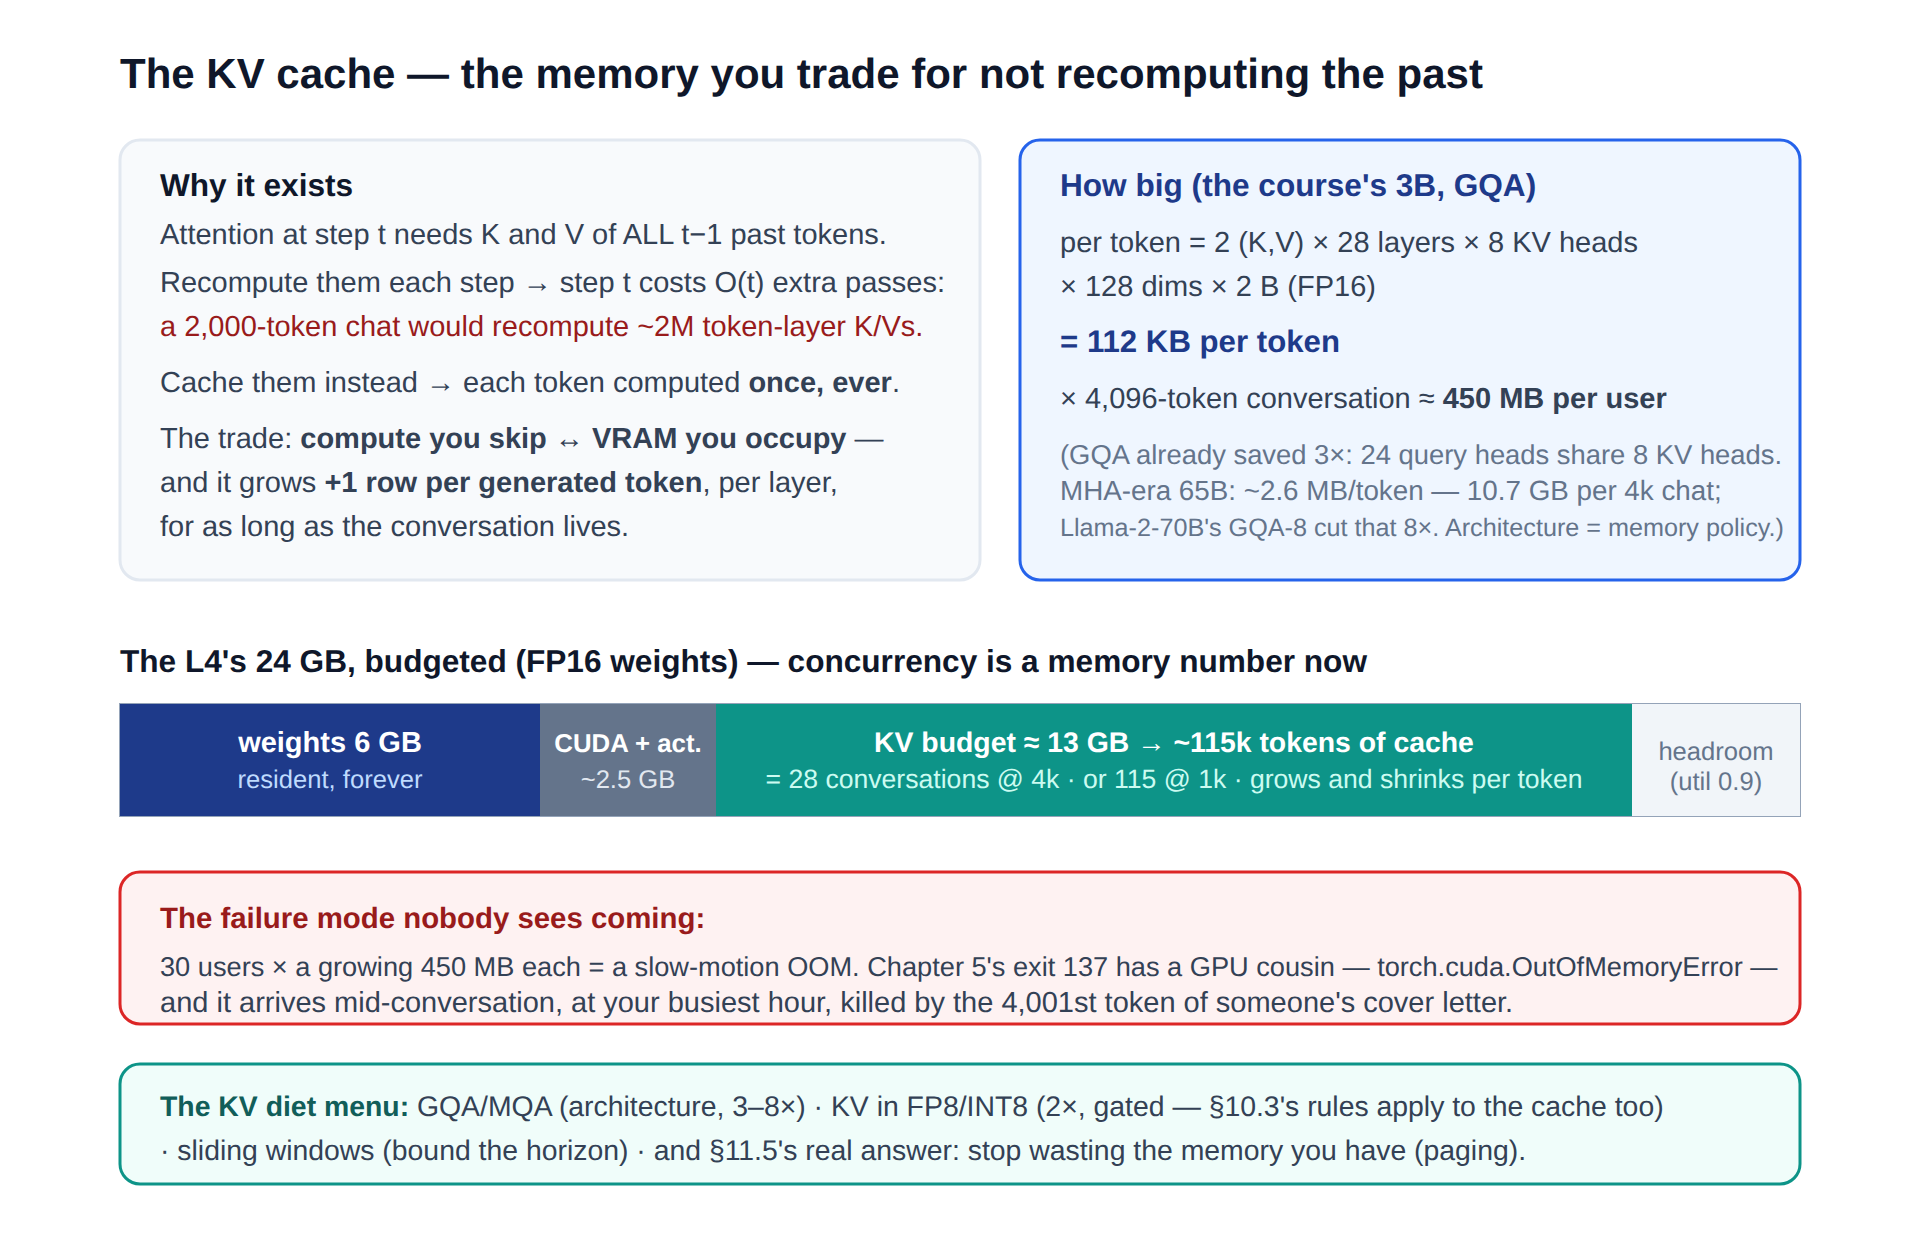
\includegraphics{figures/fig11-3_kvcache.png}}\\[3pt]
  \figcaption{Figure 11-3  Why the cache exists, what it costs per token, and the L4's 24 GB budgeted into weights, runtime, and a KV pool. GQA already cut the bill 3×; the diet menu cuts further — and §11.5 stops wasting what remains.}
\end{tbbfigure}

\subsection*{What the cache does to the decode step — the b that grows}

The cache is not only occupancy; it is \textbf{traffic}. Each decode step must \textit{read} every cached K,V the sequence owns (attention consults the whole past), so a step's bytes are: weights + the batch's total cache. Write it as Chapter 9's law with a twist — \textbf{t(step) ≈ (W\_bytes + Σ KV\_bytes(context)) ÷ bandwidth} — and run the course model at batch 32, contexts averaging 4k: bytes = 6 GB + 32 × 0.47 GB ≈ \textbf{21 GB per step → \textasciitilde{}70 ms → \textasciitilde{}14 tokens/s per stream, \textasciitilde{}460 tokens/s aggregate}. Compare batch 1: 6.47 GB → 21.5 ms → 46 tok/s. The bargain is Chapter 9's, restated for streams: \textbf{10× the aggregate throughput for 3× the per-stream latency} — and every stream still outruns its reader. But notice the new term's behavior: weights amortize across the batch (the same 6 GB serves everyone — Week 9's a), while \textbf{KV bytes scale with the batch} (each stream drags its own past — a b that grows with context). Set n × 0.47 = 6 and you find the crossover: past \textbf{\textasciitilde{}13 concurrent 4k conversations, the cache outweighs the model} — at scale, an LLM server spends more bandwidth reading conversations than reading the network that answers them.

That one computation quietly explains half the modern LLM-serving research agenda, so linger on its corollaries. \textit{Long contexts are a tax on everyone}: one 32k-token document chat drags 3.8 GB of cache through the wall \textbf{every step}, slowing all co-batched streams — length limits and context pricing are physics, not stinginess. \textit{The cache is why GQA/MQA exist} (Shazeer asked in 2019 what MHA's many KV heads were buying at inference and answered "mostly bytes"), \textit{why KV-cache quantization} is a standard lever (FP8 halves the 112 KB — §10.3's gate applies to the cache exactly as to weights), \textit{and why sliding-window models} bound the horizon outright. And it sharpens the admission problem: a new stream needs pool space \textbf{that will grow unpredictably}; when the pool fills, the engine must queue admissions or \textbf{preempt} a running stream — evict its blocks and re-prefill it later (paying compute to reclaim memory). Deciding \textit{which} — queue, preempt, or refuse — is scheduling, and scheduling is §11.4.

\subsection*{Multi-turn chat: the cache meets the stateless web}

One more consequence before the batcher, because it pays a Chapter 6 debt. HTTP APIs are stateless: each turn of a conversation re-sends the \textbf{entire history} as prompt. Mechanically that means the server re-\textit{prefills} the whole conversation every turn — turn five of a 3,000-token chat pays a 3,000-token prefill (\textasciitilde{}350 ms of pure compute) to regenerate K,V rows it computed identically four turns ago, unless someone kept them. Keeping them is called \textbf{prefix caching} (§11.5's block machinery makes it nearly free), but it resurrects Chapter 6's sticky-session tension in exact form: the kept rows live in \textbf{one replica's VRAM}, so routing turn five to a different replica silently re-pays the full prefill. Hold the tension — §11.5 resolves it the grown-up way (affinity as a \textit{performance hint}, never a correctness requirement), and the think box below makes you price both halves first.

\begin{calloutbox}{tbbpurple}{tbbpurplefill}
{\normalsize\bfseries\color{tbbpurple}Think About It}\par\vspace{3pt}
\begin{tbbitemize}
  \item Reconstruct Exhibit 11-B's timeline quantitatively: \textasciitilde{}30 conversations, each growing \textasciitilde{}2 tokens/s from a 9.8 GB floor on a 24 GB card. Predict the minute of death, then explain why the REAL curve is bumpier (hint: answers end; users pause; admissions arrive).
  \item Your PM wants a 128k-context tier "since the model supports it." Price one full 128k conversation on the course's 3B in KV bytes, in per-step traffic at batch 8, and in evicted seats — then propose the tier's price structure and its admission rule.
  \item Recompute Transcript 11-2's seat count for (a) the INT8 weights Chapter 10 shipped, (b) FP8 KV cache on top, (c) both plus GQA→MQA (1 KV head). Which single change buys the most seats, and which needs §10.3's gate most urgently?
  \item The step-cost model says a 32k document chat co-batched with 31 short chats slows everyone. Compute each stream's TPOT with and without the whale, then design the fairness policy you would actually ship (hint: per-seat KV quotas, separate pools, or pricing).
  \item Chapter 3 taught page cache as "reclaimable ballast" vs. anonymous memory as "need." Classify the KV cache: which is it — and what does your answer imply an engine may do under memory pressure that a web server never could? (§11.4's preemption is the payoff.)
\end{tbbitemize}
\end{calloutbox}

\section{Continuous Batching: The City Bus}

Batching is still the whole economy — §11.3's arithmetic said one stream leaves \textasciitilde{}97\% of the weight-stream's value unclaimed, and thirty co-riders reclaim it. So point Week 9's dynamic batcher at generation and collect the riders... and watch it die of a fine-print clause. Box 9-1 warned that dynamic batching assumes \textbf{similar-shaped requests}; Chapter 10's rule ③ taxed \textit{input} raggedness (padding) and offered bucketing. Generation breaks something bucketing cannot reach: \textbf{the outputs are ragged, and unknowably so}. Four requests enter together; the batch runs a shared decode loop; one finishes at token 32, another at 210 — and in a \textit{static} batch, the early finisher's seat rides along \textbf{dead} until the longest passenger is done, while new requests queue outside a bus full of empty seats. The numbers are not subtle: with answer lengths spread 10–100×, seat-step utilization lands near 50\%, and — crueler — an arriving request's TTFT includes the \textit{entire remaining essay} of whoever boarded before it. Exhibit 11-A's 11.4-second p99 has a second parent.

\begin{tbbfigure}
  \adjustbox{max width=0.94\linewidth,max totalheight=0.46\textheight}{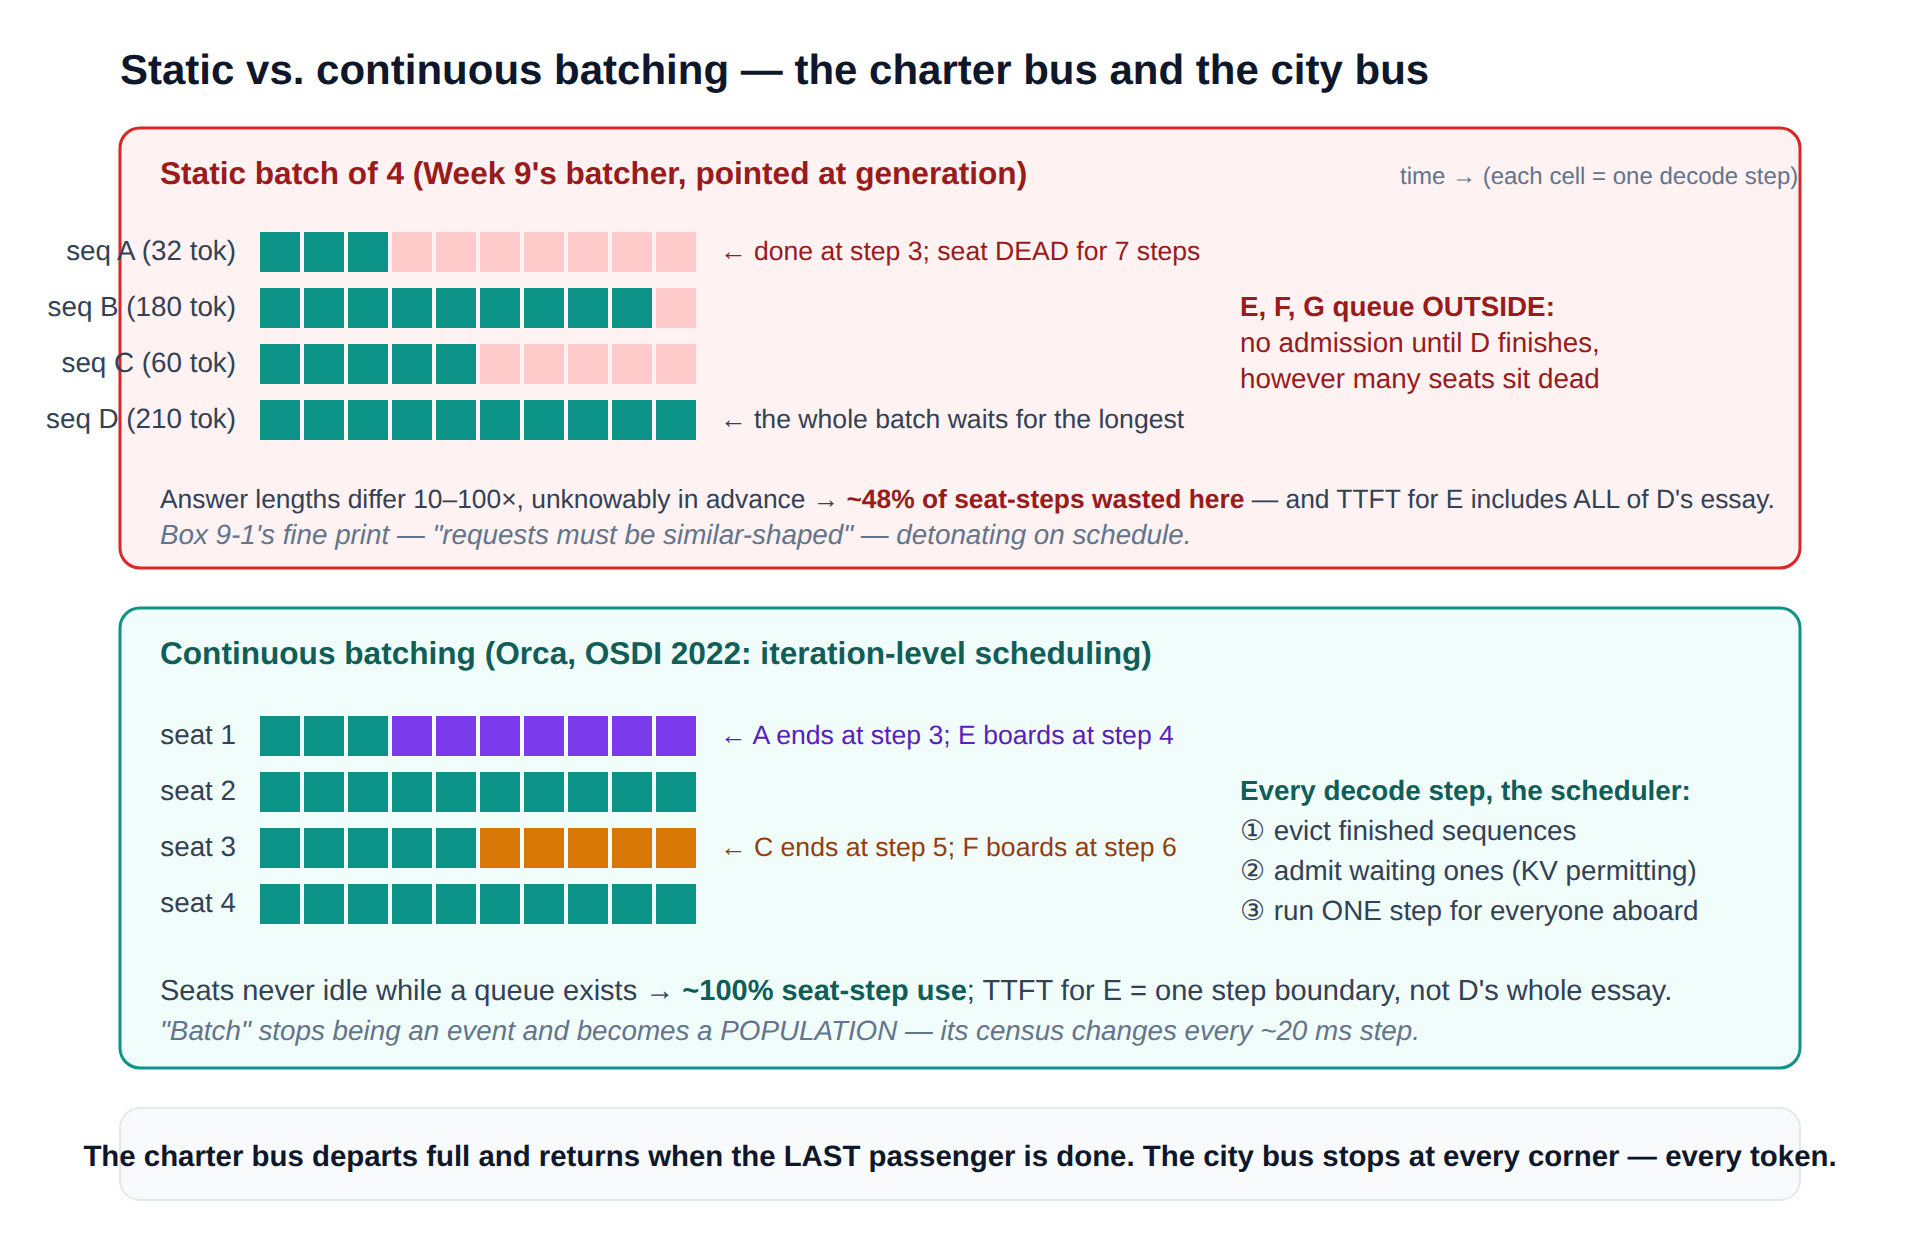
\includegraphics{figures/fig11-4_contbatch.png}}\\[3pt]
  \figcaption{Figure 11-4  The charter bus vs. the city bus. Static batching finishes together or not at all — dead seats, queued arrivals, TTFT hostage to strangers' essays. Iteration-level scheduling re-decides the manifest every \textasciitilde{}20 ms step: finished sequences leave, waiting ones board, no seat idles while a queue exists.}
\end{tbbfigure}

\subsection*{Iteration-level scheduling — Orca's one beautiful idea}

The repair (Yu et al., \textbf{Orca}, OSDI 2022 — the paper Chapter 9's further reading parked "until after the KV cache lecture," which was twenty minutes ago) is one sentence long: \textbf{stop scheduling requests; schedule iterations.} The decode loop already runs step by step — so between \textit{any} two steps, the batch's membership may change. Every \textasciitilde{}20 ms, the scheduler runs a three-beat cycle: \textbf{evict} sequences that just emitted their stop token (their seats and KV blocks free instantly); \textbf{admit} waiting sequences if the KV pool can host them (§11.3's admission rule, now load-bearing); \textbf{step} everyone aboard through one forward pass. That is continuous batching. A "batch" stops being an event with a start and an end and becomes a \textbf{population} — a census that changes at every stop. The charter bus became a city bus, and the two failure modes of Figure 11-4's top panel simply cannot occur: no seat idles while anyone queues, and a newcomer's wait is measured in \textit{steps}, not in strangers' essay lengths.

It is worth pausing on why this is \textit{possible} here and was not in Week 9. Triton's dynamic batcher could not evict-and-admit mid-flight because a CNN's forward pass is \textbf{one indivisible kernel} launch: there is no "between steps" to intervene in. Generation's inefficiency — an outer Python-visible loop, one step per token — turns out to be scheduling's opportunity: the loop's seams are where the scheduler lives. (Orca's second contribution, \textit{selective batching}, handles the tensor plumbing of ragged co-resident sequences: attention runs per-sequence against per-sequence caches, while the fat linear layers batch across everyone. vLLM's kernels inherit the pattern.) One more Week 9 souvenir survives translation: \textbf{max\_queue\_delay is gone} — there is nothing to wait for, since the next departure is at most one step away. Its successor knob is \textit{how much work rides one step}, and that knob is where the two clocks start fighting.

\subsection*{Prefill–decode interference: the two clocks, one engine}

Admitting a new stream is not free seat assignment: the newcomer needs its \textbf{prefill} — 50–350 ms of compute-bound GEMM — executed by the same GPU that thirty decode streams are using in 20 ms sips. Run the prefill as one indivisible step and everyone's next token waits behind it: thirty streams \textbf{hiccup} — TPOT spikes from 21 to \textasciitilde{}250 ms, a stutter the reader's eye actually catches — so that one newcomer's TTFT could be minimal. Delay prefills instead and TTFT bloats while decode purrs. This is the serving triangle reborn with new corner names: \textbf{TTFT vs. TPOT vs. cost}, and the knob that walks the edge is \textbf{chunked prefill}: slice the 500-token prefill into (say) four chunks and co-schedule one chunk per decode step, so the newcomer's prefill completes over four steps (TTFT +\textasciitilde{}60 ms) while incumbents' TPOT rises only \textasciitilde{}2 ms per step. Engines expose the trade as a budget — vLLM's \code{max\_num\_batched\_tokens} caps \textit{total tokens (prefill chunks + decode steps) per iteration} — and tuning it is the §9.3 knob-sweep reborn, now with two latency clocks on the report instead of one.

\begin{terminalbox}
\begin{Verbatim}[breaklines=true,breakanywhere=true,fontsize=\small,formatcom=\color{tbbtermfg},codes=\tbbcodeactive]
# vLLM /metrics, sampled every 30 s while load ramps (c = 4 -> 64):
$ watch -n 30 'curl -s :8000/metrics | grep -E "running|waiting|cache"'

#            running   waiting   gpu_cache_usage    <- read as:
t+0:00          4          0          9 %           # roomy. TTFT=prefill
t+1:30         19          0         41 %           # filling. all admitted
t+3:00         31          0         88 %           # full-ish. TPOT sagging
t+4:30         32          9         97 %           # pool full: queue forms
t+6:00         32         26         98 %           # waiting grows: TTFT now
                                                    # queue-dominated (L=λW!)
# the three regimes every LLM service lives in: ROOMY (TTFT=prefill),
# FULL (TPOT shares bandwidth), QUEUED (TTFT explodes first).
# your SLO breaks in regime 3 at the TTFT clause - almost never TPOT.
\end{Verbatim}
\end{terminalbox}
\figcaption{Transcript 11-3  Continuous batching, watched through its own metrics. running climbs to the KV-pool seat count and stops; waiting appears the moment the pool fills; and the failure sequence under load is always the same — TTFT dies first, by queueing, exactly as Chapter 7's hockey stick predicts.}

\subsection*{What the knobs became — Week 9's sweep, translated}

\begin{tbbtablewrap}
  \begin{tabular}{@{}>{\raggedright\arraybackslash}m{\dimexpr 0.2447\tbltextwidth-2\tabcolsep\relax} >{\raggedright\arraybackslash}m{\dimexpr 0.2660\tbltextwidth-2\tabcolsep\relax} >{\raggedright\arraybackslash}m{\dimexpr 0.4894\tbltextwidth-2\tabcolsep\relax}@{}}
  \arrayrulecolor{tbbnavy}\specialrule{1pt}{0pt}{0pt}
  \rowcolor{tbbtablehead}{\centering \bfseries\color{tbbnavy}Week 9 (dynamic batching)} & {\centering \bfseries\color{tbbnavy}Week 11 (continuous batching)} & {\centering \bfseries\color{tbbnavy}What changed, and why} \\
  \arrayrulecolor{tbbnavy}\specialrule{0.7pt}{0pt}{2pt}
  {max\_batch\_size} & {\textbf{max\_num\_seqs}} & {Seat count — but the KV pool usually binds first (§11.3); this mostly caps worst-case interference} \\
  \arrayrulecolor{tbbtableborder}\hline
  {max\_queue\_delay} & {\textbf{(gone)}} & {Nothing to wait for: the next departure is one step (\textasciitilde{}20 ms) away — the knob died of success} \\
  \arrayrulecolor{tbbtableborder}\hline
  {(no equivalent)} & {\textbf{max\_num\_batched\_tokens}} & {The step budget: prefill chunks + decode tokens per iteration — the TTFT ↔ TPOT dial} \\
  \arrayrulecolor{tbbtableborder}\hline
  {memory.max (Ch. 5, outside)} & {\textbf{gpu\_memory\_utilization}} & {The limit moved inside the engine and inverted: grant a budget, the engine derives its own seat count} \\
  \arrayrulecolor{tbbtableborder}\hline
  {(crash on overflow)} & {\textbf{preemption policy}} & {The overdraft plan: evict a sequence's blocks and recompute later — memory reclaimed by spending compute} \\
  \arrayrulecolor{tbbnavy}\specialrule{1pt}{2pt}{0pt}
  \end{tabular}\par
  \figcaption{Table 11-1  The batcher's panel, translated. Every Week 9 instinct has a Week 11 home — but the units moved from requests to tokens, and the binding resource moved from compute to the KV pool.}
\end{tbbtablewrap}

The §9.3 batcher had two knobs; the continuous batcher's panel translates them. \textbf{max\_num\_seqs} (seat count) succeeds max\_batch\_size — but §11.3 showed the real bound is usually the KV pool, so this knob mostly caps worst-case interference. \textbf{max\_num\_batched\_tokens} (step budget) succeeds max\_queue\_delay as the TTFT↔TPOT dial. \textbf{gpu\_memory\_utilization} sizes the pool itself — Chapter 5's memory.max discipline, now \textit{inside} the engine and, pleasingly, inverted: instead of measuring worst-case usage and setting a limit, you \textit{grant} a budget and the engine computes its own seat count. And \textbf{preemption policy} handles the pool's overdraft: vLLM evicts a whole sequence's blocks and \textbf{recomputes} its prefill later when space frees (paying compute to reclaim memory — your Ch. 3 think-box answer, industrialized; swapping blocks to host RAM exists too, but §10.2's PCIe arithmetic explains why recompute usually wins). The lab's sweep (§11.6) walks exactly this panel, and the deliverable is the same as every sweep since Week 9: the knee, found on purpose, written down.

Preemption deserves one look in the flesh, because you will meet it as a log line before you meet it as a concept — and misread it as an error if this paragraph doesn't get there first:

\begin{terminalbox}
\begin{Verbatim}[breaklines=true,breakanywhere=true,fontsize=\small,formatcom=\color{tbbtermfg},codes=\tbbcodeactive]
# push admission past the pool on purpose (c=48, long answers) and
# watch the engine's overdraft plan execute:
WARNING  Sequence group chatcmpl-8f21 is preempted by
         PreemptionMode.RECOMPUTE because there is not enough KV
         cache space. total_num_cumulative_preemption=1
INFO     Avg generation throughput: 691.2 tokens/s,
         Running: 31 reqs, Waiting: 17 reqs, GPU KV cache usage: 99.8%
# not a crash: one conversation's blocks were evicted; it will
# re-prefill when space frees. the victim's next tokens stall ~400 ms.
# occasional = healthy elasticity. CONSTANT = your pool is undersized:
# quantize the weights, shrink max-model-len, or buy the bigger card.
\end{Verbatim}
\end{terminalbox}
\figcaption{Transcript 11-4  Preemption, live. The WARNING is the design working — Chapter 3's OOM killer had no gentler option; the block manager does: evict, queue, re-prefill. Read the counter like a vital sign: near-zero is elastic, climbing is undersized.}

One honest boundary: continuous batching optimizes \textit{throughput under raggedness}; it does not repeal §11.3's bandwidth arithmetic (TPOT still degrades \textasciitilde{}3× from batch 1 to batch 32 — the riders share one memory bus), and it cannot help the workload with \textbf{no co-riders} — a single user's agent loop, batch-1 forever, remains the memory wall's prisoner and is precisely the case §11.5's speculative decoding exists for. The engine's gift is narrower and immense: it guarantees the \textit{seats you paid for are never empty while anyone is waiting}. Whether the seats are cheap enough is still Chapters 10 and 12's business.

\begin{calloutbox}{tbbpurple}{tbbpurplefill}
{\normalsize\bfseries\color{tbbpurple}Think About It}\par\vspace{3pt}
\begin{tbbitemize}
  \item Static batch of 4, answer lengths 32/180/60/210 tokens (Figure 11-4). Compute exact seat-step waste, the TTFT of a request arriving at step 10, and both numbers under continuous batching. Then explain why bucketing-by-INPUT-length (Ch. 10 rule ③) fixes none of it.
  \item Chunked prefill with a 2,000-token prompt, chunk = 512 tokens, decode step ≈ 21 ms, prefill chunk ≈ 55 ms co-scheduled: estimate the newcomer's added TTFT and the incumbents' TPOT during the four mixed steps. Now argue the OTHER side: when would you deliberately run whole-prompt prefills (hint: a dedicated prefill replica — DistServe's idea, Box 11-1)?
  \item Transcript 11-3's regime 3 shows waiting=26 with running pinned at 32. Using L = λW with W ≈ 4.4 s, estimate the arrival rate, the queue's growth rate, and the TTFT of the 26th waiter. Which SLO clause reports the failure, and what does Chapter 12 sell to fix it?
  \item vLLM preempts by evict-and-recompute. Price a preemption of a 3,000-token conversation in (a) wasted prefill compute, (b) the victim's next-turn TTFT, (c) fairness. Design the policy: whom do you preempt — newest, longest, or cheapest-to-recompute — and defend it to the victim.
\end{tbbitemize}
\end{calloutbox}

\section{PagedAttention and vLLM: The OS Moves Inside}

Everything so far says seats are precious: §11.3 priced them in KV bytes, §11.4 promised none would idle. So it should sting to learn how the pre-2023 engines \textit{stored} the cache: one \textbf{contiguous slab per sequence, sized for the maximum possible length}, allocated at admission. Contiguous, because attention kernels wanted clean strides; max-sized, because nobody knows at admission whether the answer will run 30 tokens or 3,000. You have seen this movie — it is malloc's oldest tragedy, and it played out exactly on schedule: \textbf{internal waste} (the reserved-but-unused tail of every slab — reserve 2,048, use 180, waste 91\%) plus \textbf{external fragmentation} (freed slabs leave gaps that fit no new max-sized request). When the vLLM authors measured production-grade systems for their SOSP 2023 paper, the number was damning: \textbf{60–80\% of KV memory held nothing useful}. Your hard-won 13 GB pool, behaving like 4. More than half the bus's seats, dismantled for storage of air.

\begin{tbbfigure}
  \adjustbox{max width=0.94\linewidth,max totalheight=0.46\textheight}{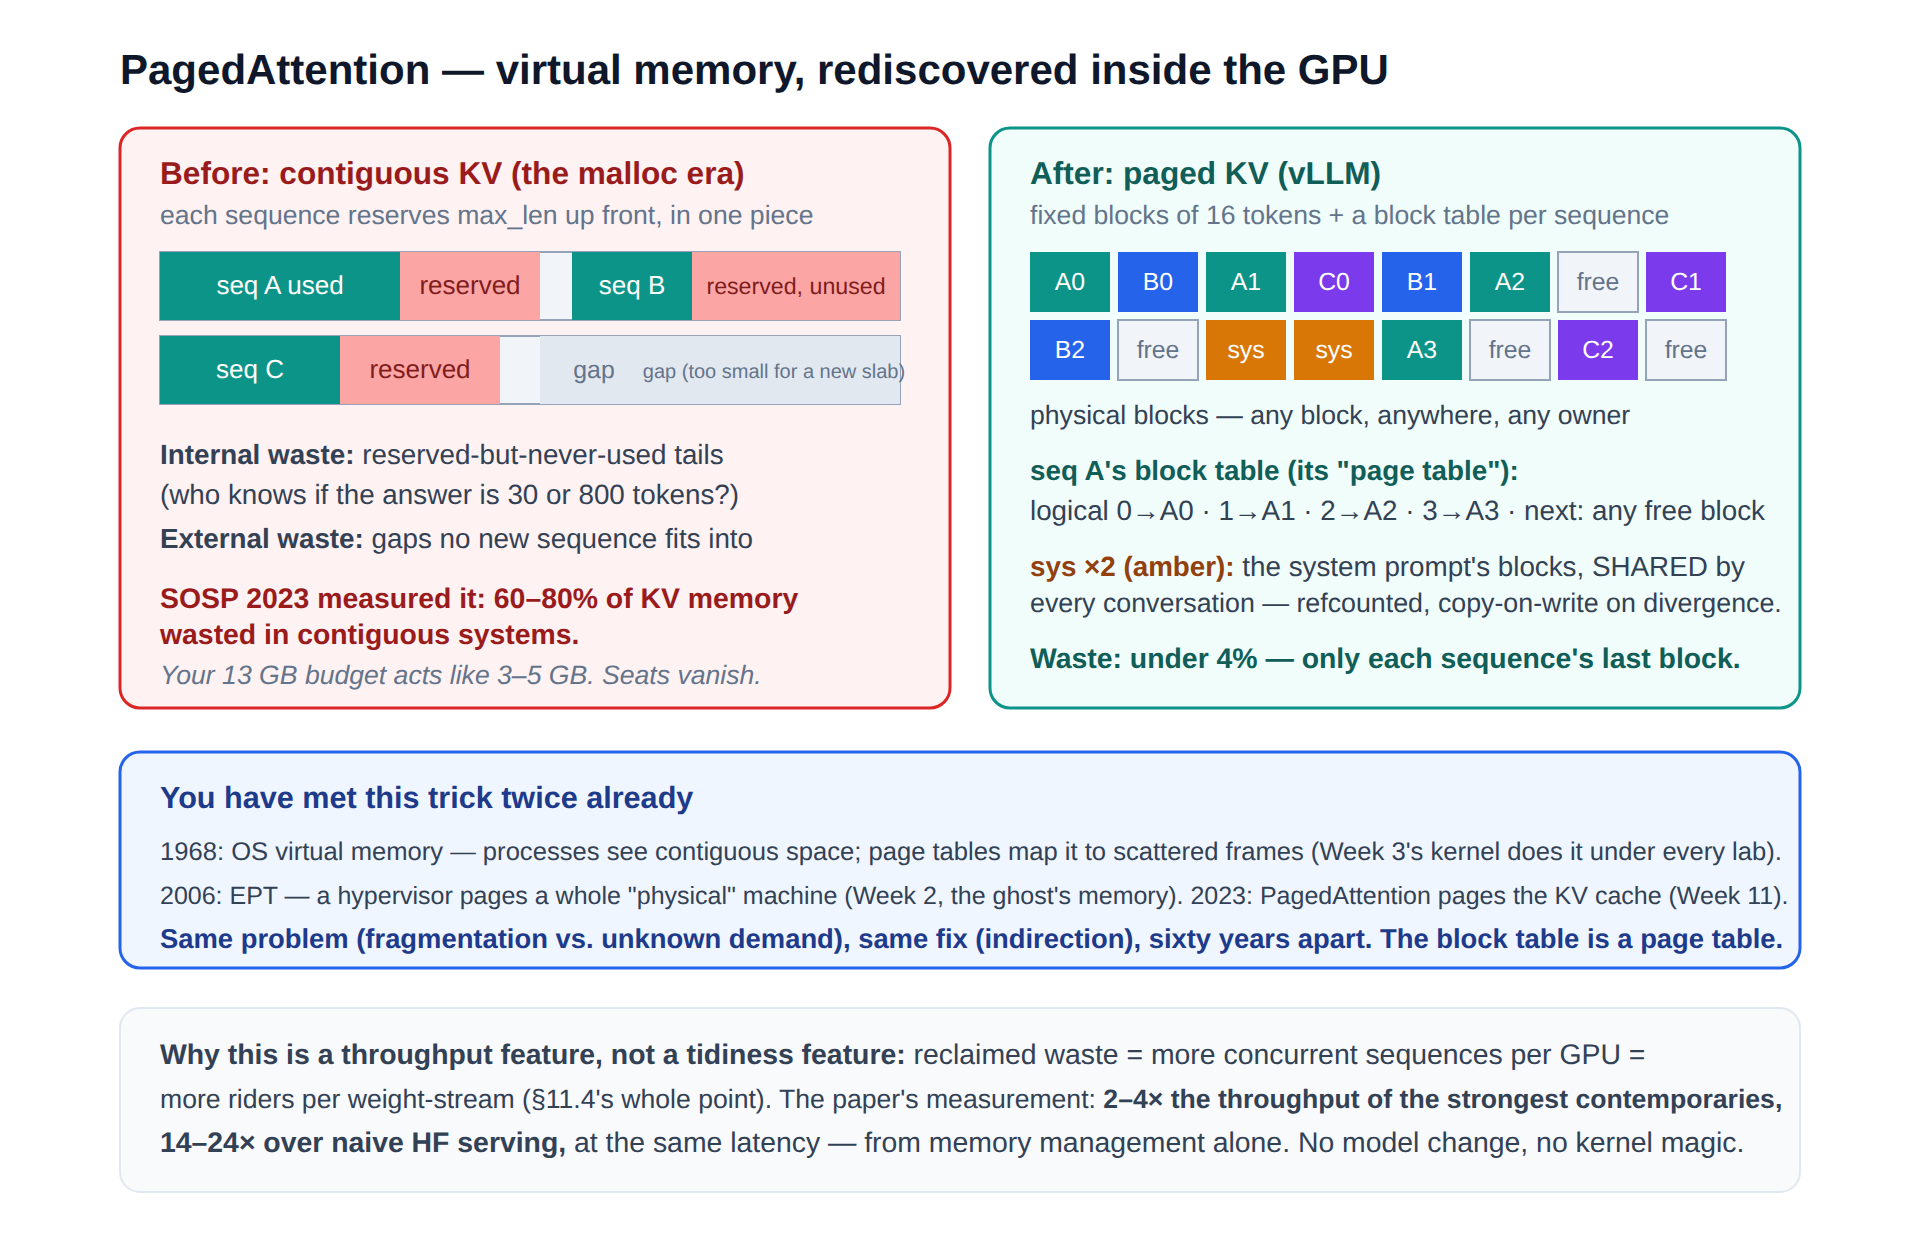
\includegraphics{figures/fig11-5_paged.png}}\\[3pt]
  \figcaption{Figure 11-5  The malloc era vs. the paged era. Contiguous max-length slabs waste 60–80\% of the pool between reservation tails and unusable gaps; fixed 16-token blocks plus per-sequence block tables cut waste under 4\% — and make sharing a refcount instead of a copy.}
\end{tbbfigure}

\subsection*{The sixty-year-old fix, applied at 300 GB/s}

The fix is the most successful indirection trick in computing history, and this course has already shown it to you twice. Operating systems stopped giving processes contiguous physical memory in the 1960s: they hand out fixed-size \textbf{pages}, let a \textbf{page table} translate the process's tidy virtual addresses onto scattered physical frames, and fragmentation collapses to "part of the last page." Week 3's kernel does this beneath every lab you have run; Week 2 showed the trick \textit{stacked} — EPT paging an entire guest's "physical" memory as though it were one more process. \textbf{PagedAttention} (Kwon et al., SOSP 2023 — the paper Chapter 1 flagged as required reading, and the reason this course teaches vLLM) transplants it whole into attention: chop the KV pool into fixed blocks of \textbf{16 tokens}; give each sequence a \textbf{block table} mapping logical position → physical block; teach the attention kernel to follow the table. A sequence now grows one \textit{block} at a time, blocks live anywhere, and waste shrinks to each sequence's half-full final block — the paper measured \textbf{under 4\%}. No model change, no precision change: bookkeeping. And the throughput consequence is Chapter-10-sized \textit{because seats compound}: reclaimed waste → 2–3× more concurrent sequences in the same pool → that many more riders amortizing every 20 ms weight-stream. Measured end to end: \textbf{2–4× the throughput of the strongest contemporary systems, 14–24× over naive HF serving, at equal latency}. The best systems paper of its serving generation is, at heart, a memory allocator — which is precisely the sensibility this course has been selling since the cgroup chapter.

\subsection*{Sharing: the block table's second trick — and Chapter 6's debt, paid}

Page tables did more for the OS than kill fragmentation — two processes mapping the same physical frame gave Unix shared libraries and copy-on-write fork. The block table replays that too. Every conversation in your product begins with the same \textbf{900-token system prompt}; contiguous slabs stored it 32 times (32 × 900 × 112 KB ≈ \textbf{3.2 GB of identical bytes} — nearly seven 4k-seats of pure duplication). Paged, those 900 tokens are \textasciitilde{}57 blocks with a \textbf{reference count}: every conversation's table points at the \textit{same} physical blocks, storing them \textbf{once} (≈ 101 MB); a sequence that diverges gets \textbf{copy-on-write} at block granularity. This is \textbf{prefix caching}, and it pays twice: the memory (6+ seats reclaimed) and the \textit{clock} — a new conversation whose prefix is already resident \textbf{skips that prefix's prefill entirely}, cutting \textasciitilde{}100 ms of compute out of TTFT; a returning conversation's turn five re-prefills only the new suffix, not the 3,000-token history (§11.3's multi-turn tax, mostly refunded).

Which resolves the sticky-session tension Chapter 6 told you to hold. The cached blocks live in \textbf{one replica's VRAM} — so should the router pin conversations to replicas? The grown-up answer the industry converged on: \textbf{correctness stays stateless; affinity is a performance hint.} The request still carries full history, so \textit{any} replica can serve turn five correctly — a cache miss costs one suffix... one \textit{full} prefill (\textasciitilde{}350 ms), never a wrong answer. Given that, session-hash routing (consistent-hash on conversation id) is pure upside \textit{when convenient} and harmlessly degradable when not: a rollout, a scale-down, or a replica death (Ch. 6's three horsemen of sticky state) merely dents the prefix-hit rate for a minute. Contrast the design Chapter 6 warned against — a session \textit{store} whose loss breaks conversations. Same word, "sticky"; opposite engineering: \textbf{never let a cache become a contract.}

\subsection*{vLLM, organ by organ — and the speculation lever}

Assemble the chapter and you get vLLM's block diagram (Figure 11-6), which is Chapter 9's six-organ anatomy with two organs transplanted: the \textbf{batcher} is §11.4's iteration scheduler; the \textbf{model store}'s hot path grew an in-VRAM "OS" — the block manager — running §11.5's tables, refcounts, and preemption. Around them, the familiar: an OpenAI-compatible front door speaking SSE (so every client, LB, and timeout lesson from Chapter 6 applies verbatim), Chapter 6's safetensors loading, Prometheus metrics whose names you already read in Transcript 11-3. Inside the executor, two Chapter 10 callbacks earn their keep: decode steps are captured as \textbf{CUDA Graphs} — a 3B decode step is hundreds of small kernels in a 21 ms budget, so launch overhead is a first-class enemy and the graph replays the whole step as one submission (Chapter 10's \textit{a}, crushed at runtime rather than build time) — and the weights slot accepts the \textbf{GPTQ/AWQ INT4} artifacts whose per-group-scale vocabulary Chapter 10 taught: the course model at INT4 is \textasciitilde{}1.9 GB, dropping the batch-1 step to \textasciitilde{}2.4 GB of traffic → \textbf{\textasciitilde{}8 ms → 2.5× the tokens/s}, \textit{and} widening the KV pool by 4 GB (≈ 9 more 4k-seats). Both clocks and the seat count, one gated artifact — §10.3's gate (perplexity or task metric vs. a written tolerance) applies unchanged.

One executor line deserves its own paragraph, because it pays Chapter 10's last IOU and bends §11.2's "inherently serial" rule: \textbf{speculative decoding}. The insight is an arbitrage on the memory wall's asymmetry: a decode step's 20 ms buys the \textit{bandwidth} of one token but the \textit{FLOPs} of hundreds (AI ≈ 1 against a ridge of 400 — the compute is already paid for and idle). So let a tiny \textbf{draft model} (say \textasciitilde{}160M: \textasciitilde{}1 ms/token) guess k = 4 tokens cheaply, then have the target model \textbf{verify all four in one pass} — which streams the same 6 GB as generating \textit{one} token. Accept the longest correct prefix (sampling-corrected so the output distribution is \textit{provably unchanged} — this is a systems trick, not a quality trade); on typical text \textasciitilde{}3 of 4 survive. Effective cost: (4 × 1 ms draft) + (one 21.5 ms verify) ≈ 25.5 ms for \textasciitilde{}3 tokens → \textbf{\textasciitilde{}8.5 ms/token, a 2.5× TPOT win at batch 1}, bought entirely with FLOPs that were going to waste. The honest fine print: acceptance collapses on hard or unusual text (speedup → 1× while still paying the draft), the draft occupies VRAM, and at high batch the idle-FLOPs subsidy shrinks — which is why speculation is the \textit{single-user agent loop's} lever, roughly complementary to continuous batching's many-users lever.

\begin{calloutbox}{tbbpurple}{tbbxF5F3FF}
{\normalsize\bfseries\color{tbbx5B21B6}Box 11-1  The wider LLM-serving menu — levers this course leaves on the shelf}\par\vspace{3pt}
Chapter 12 needs your remaining weeks, so these get honest one-liners instead of sections — enough to recognize the idea and its price when you meet it:

\begin{tbbitemize}
  \item \textbf{Disaggregated prefill (DistServe-style):} run prefill and decode on \textit{separate replica pools} — the two machines of §11.2, physically separated so they cannot interfere; the price is shipping the prefilled KV cache across the network between them (§10.2's PCIe lesson, cluster edition).
  \item \textbf{Multi-LoRA serving:} dozens of fine-tuned adapters sharing one base model's weights and KV pool — the S-LoRA trick; adapters are megabytes, so "one model per customer" stops meaning "one GPU per customer."
  \item \textbf{Structured/guided decoding:} constrain sampling with a grammar or JSON schema (token masks per step) — output validity for agent pipelines, at a small per-step mask cost; SGLang's RadixAttention pairs it with aggressive prefix reuse across program-shaped calls.
  \item \textbf{KV offload \& tiering:} spill cold conversations' blocks to host RAM or NVMe and restore on the next turn — trading §10.2's PCIe bytes against §11.3's re-prefill compute; the block table makes it a paging policy, literally.
\end{tbbitemize}

Every one of them is a remix of this chapter's three primitives — the two-phase loop, the block table, the iteration scheduler. Learn the primitives; the products date, the primitives don't.
\end{calloutbox}

\vspace{3.0pt}

\begin{tbbfigure}
  \adjustbox{max width=0.94\linewidth,max totalheight=0.46\textheight}{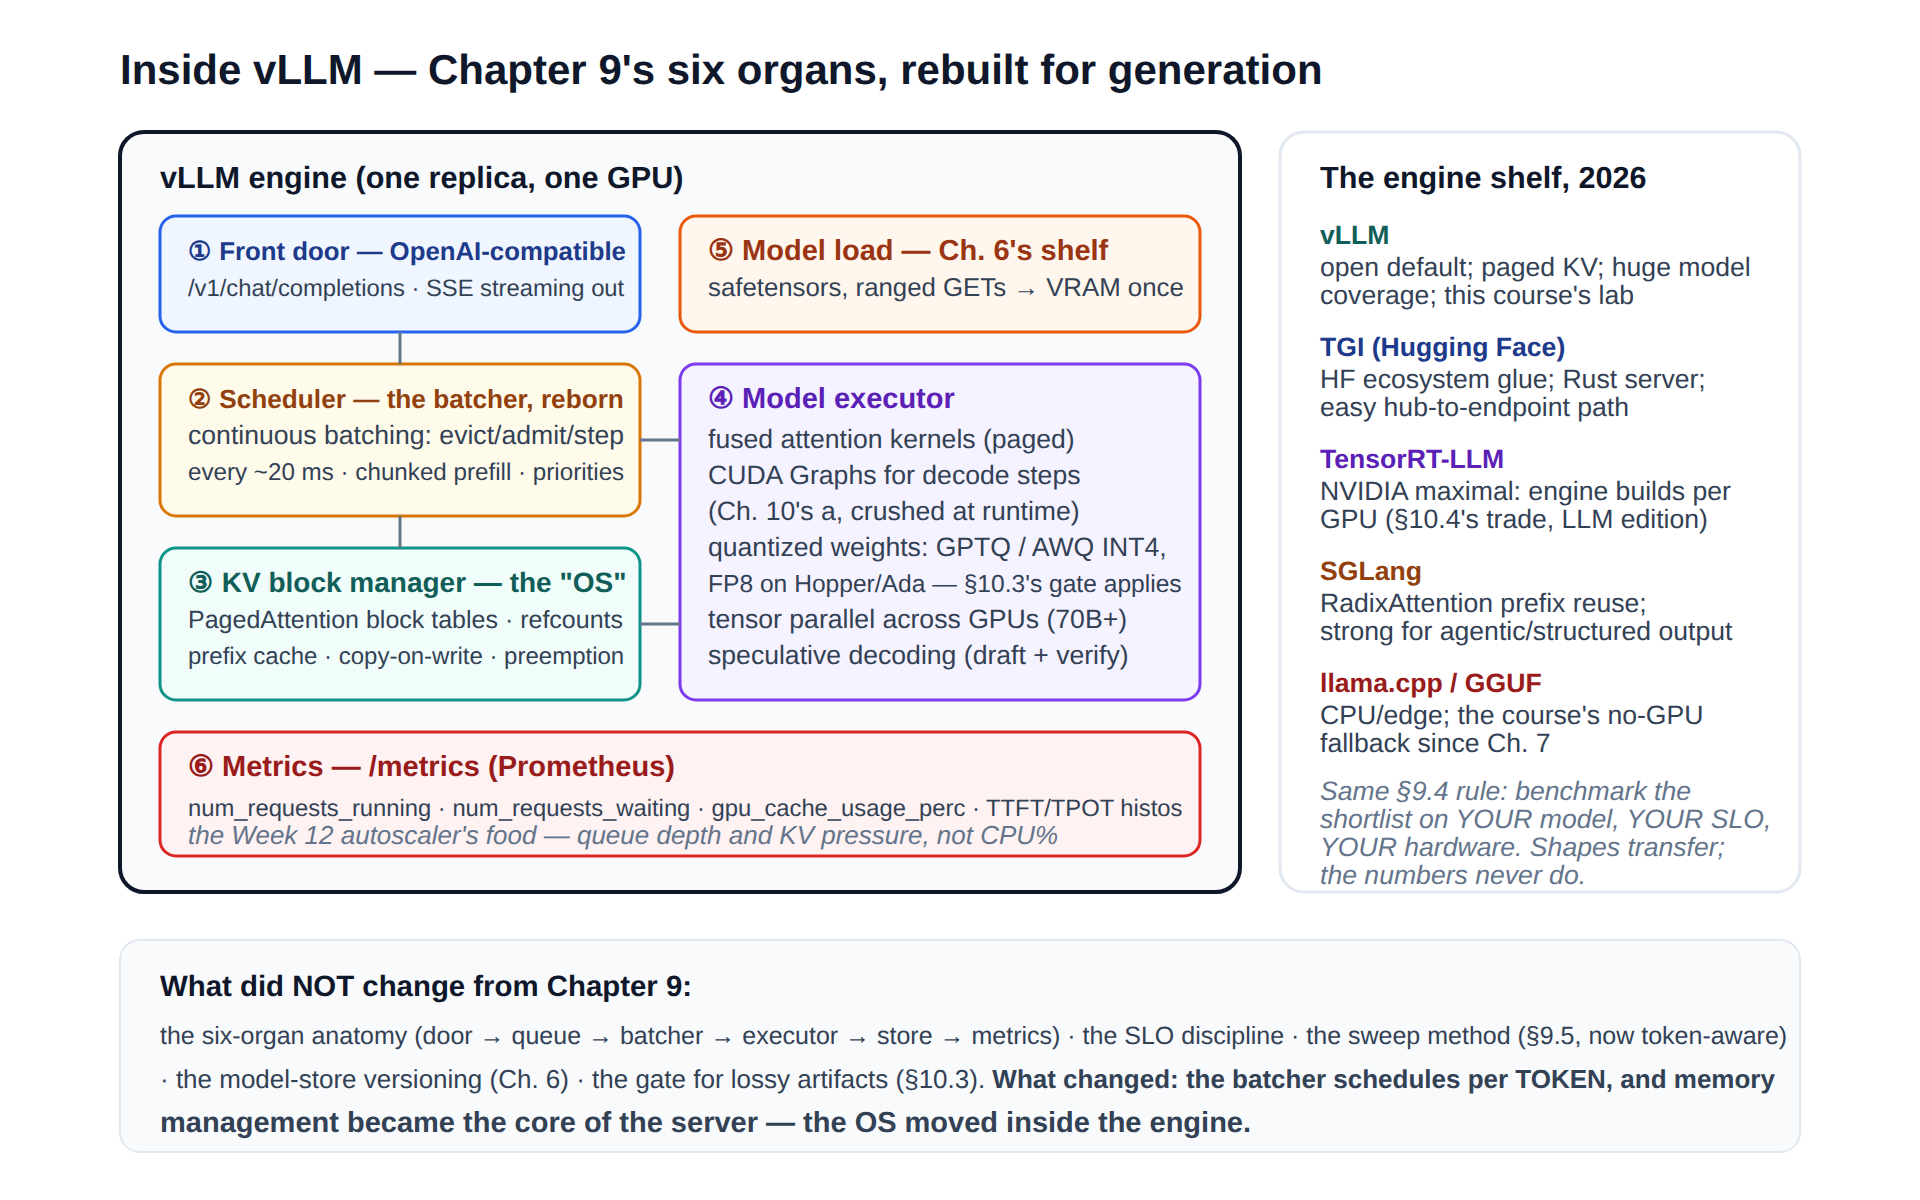
\includegraphics{figures/fig11-6_vllm.png}}\\[3pt]
  \figcaption{Figure 11-6  vLLM as Chapter 9's anatomy, rebuilt: the batcher schedules per token, the block manager runs a page table, and the metrics feed Week 12's autoscaler. Right: the 2026 engine shelf — same §9.4 rule: benchmark the shortlist on your model, your SLO, your hardware.}
\end{tbbfigure}

The shelf around vLLM (Figure 11-6, right) gets Chapter 9's treatment in miniature. \textbf{TGI} is Hugging Face's glue — the shortest hub-to-endpoint path inside that ecosystem. \textbf{TensorRT-LLM} is §10.4's trade at LLM scale: per-GPU engine builds buying maximal kernels, narrowness included; it is where \textbf{FP8} earns its keep on Hopper/Ada silicon (weights \textit{and} KV cache — Table 10-1's "Week 11's FP8 lives here," arrived; the fleet's L4 has the circuits, and the same §10.3 gate governs). \textbf{SGLang} leads when calls look like programs (agents, heavy shared prefixes, schema-bound output). \textbf{llama.cpp/GGUF} remains the course's no-GPU fallback since Chapter 7. The choosing rule has not changed since §9.4 and never will: \textit{benchmark the shortlist on your model, your SLO, your hardware — shapes transfer, numbers don't.} This course labs on vLLM because it is the open default, its metrics teach the concepts, and its paper is the chapter.

\begin{calloutbox}{tbbpurple}{tbbpurplefill}
{\normalsize\bfseries\color{tbbpurple}Think About It}\par\vspace{3pt}
\begin{tbbitemize}
  \item Compute the fragmentation waste for a contiguous engine serving answers uniform in [30, 2,000] tokens with max\_len 2,048 slabs: expected internal waste per sequence, and the seats lost on the L4's 13 GB pool vs. paged blocks of 16. Then explain why block size 16 (not 1, not 512) — what does each extreme cost?
  \item Your product A/B test shows prefix caching cut mean TTFT by 38\% but p99 TTFT by only 6\%. Explain both numbers with §11.4's regimes and the hit-rate distribution across replicas — and say what routing change (one line in the LB config) most improves the p99.
  \item Speculative decoding is "provably distribution-preserving," yet §10.3 demanded a gate for every lossy change. Is speculation lossy? What SHOULD you still verify before shipping it (think: latency distribution, cost per token, acceptance-rate telemetry), and what dashboard line detects its silent failure mode?
  \item Design multi-LoRA admission for one L4: base 6 GB, adapters 40 MB each, KV pool shared. A customer's adapter has a 300-token system prefix (cacheable). Where do the seats go as adapter count grows — and at what point does "one base, many adapters" beat "quantize the base and buy more seats"? Sketch the arithmetic.
\end{tbbitemize}
\end{calloutbox}

\section{Lab: Serve, Stream, and Measure a Real LLM}

This lab has a different texture from Weeks 9 and 10: nothing needs building — vLLM is one \code{pip install} — so \textbf{every minute goes to measurement}, and the deliverable is the project's new SLO sentence with numbers under it. You will serve a small open model on the course T4 (Qwen2.5-1.5B-Instruct: ungated, 3.1 GB in FP16, comfortable beside its KV pool in 16 GB), stream it with your own eyes, then do to the two clocks what Week 9 did to the one. Budget: \textasciitilde{}\$2–3 of GPU time; the ritual billing screenshot survives, as ever.

\begin{tbbfigure}
  \adjustbox{max width=0.94\linewidth,max totalheight=0.46\textheight}{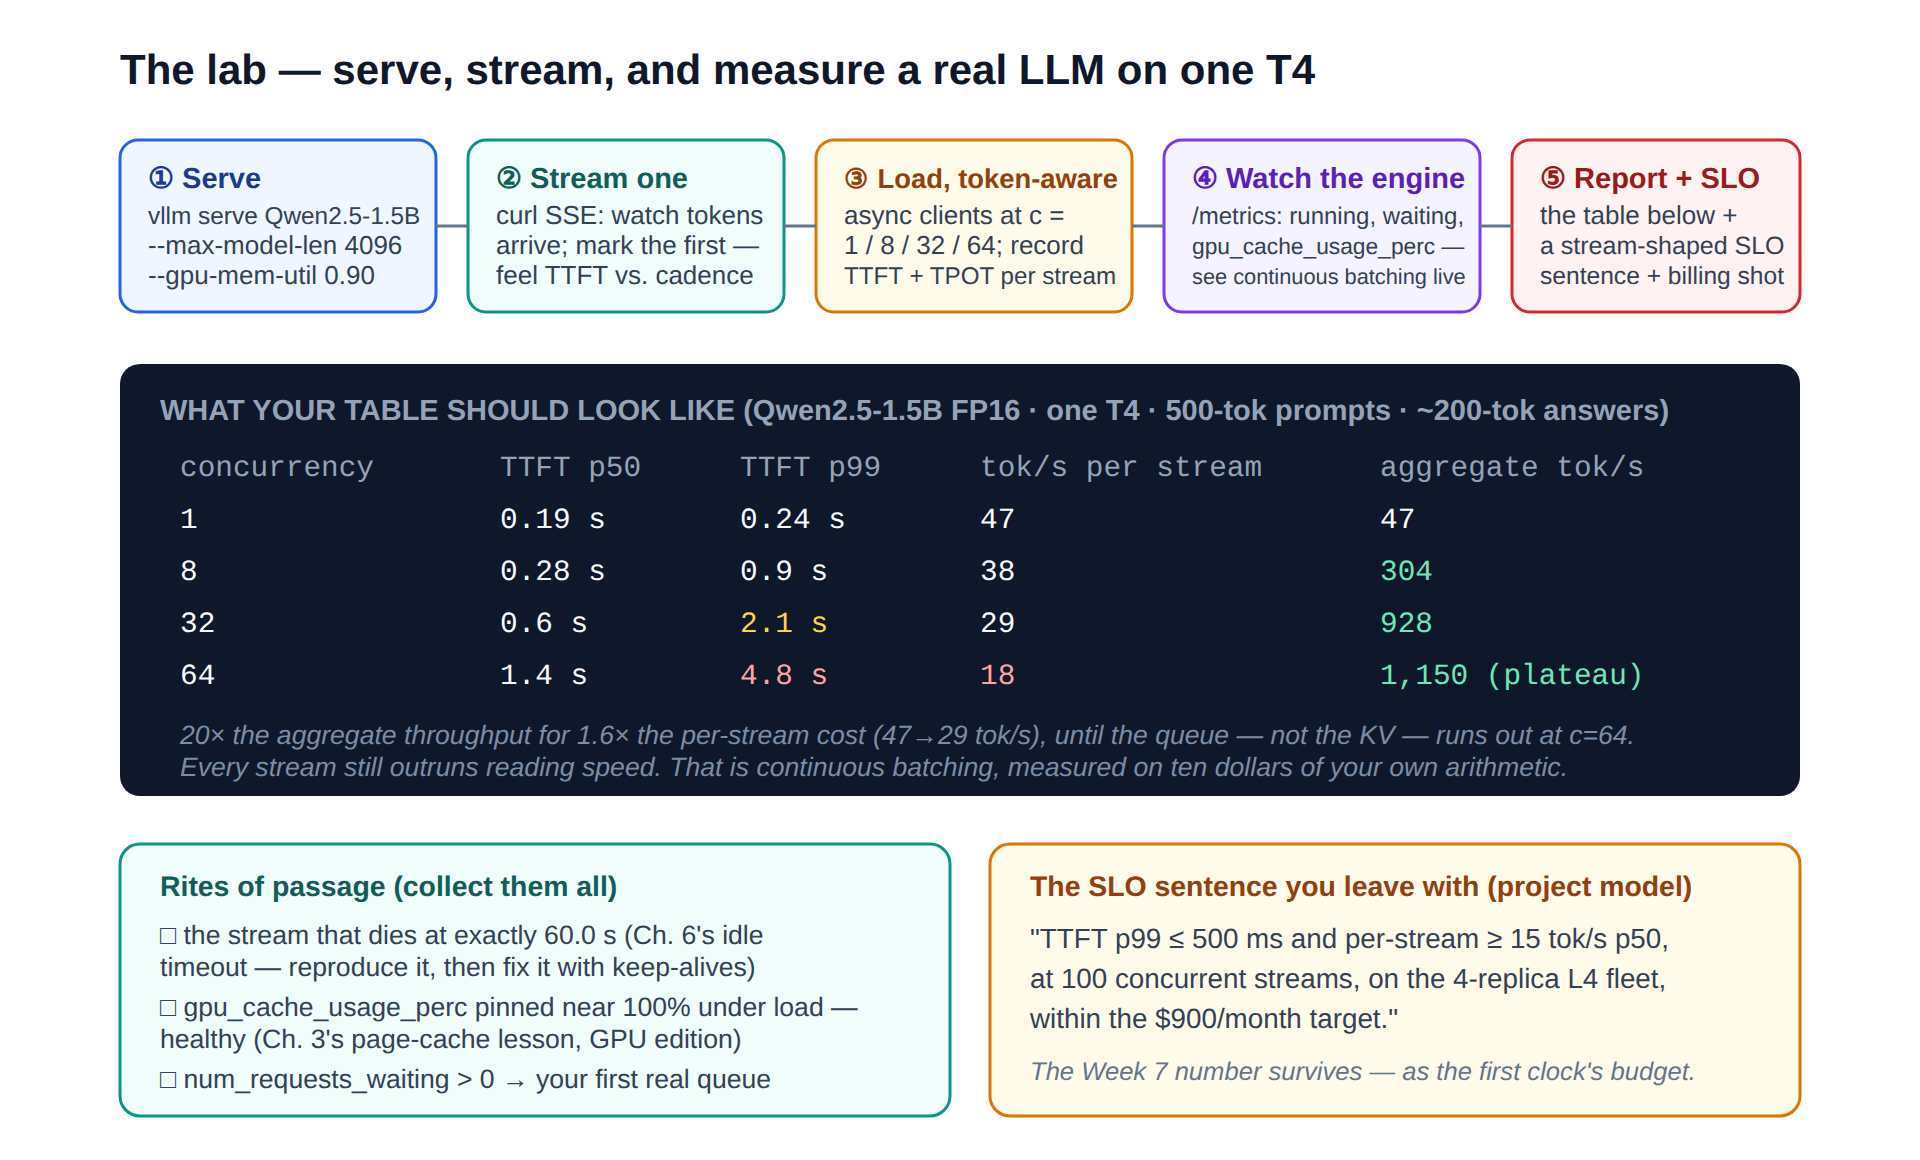
\includegraphics{figures/fig11-7_lab.png}}\\[3pt]
  \figcaption{Figure 11-7  The lab's pipeline and its expected shape: serve, stream one by hand, load-test token-aware, watch the engine's own census, and leave with the table, the SLO sentence, and two collected rites of passage.}
\end{tbbfigure}

\subsection*{The seven steps}

\begin{tbbitemize}
  \item \textbf{① Serve it.} \code{vllm serve Qwen/\allowbreak Qwen2.5-1.5B-Instruct --max-model-len 4096 --gpu-memory-utilization 0.90}. Read the boot log like a systems person: weight load (Ch. 6's ranged GETs), CUDA graph capture (Ch. 10's a), and the line that prints \textbf{how many KV blocks the pool holds} — Transcript 11-2's arithmetic, done for you by the engine. Startup takes a minute-plus: your Ch. 5 readiness probe budget, remembered.
  \item \textbf{② Stream one, by hand.} Transcript 11-5: \code{curl -N} with \code{"stream": true}, and \textit{watch} the SSE chunks arrive — first chunk after a breath (TTFT), then a steady drizzle (TPOT). You are looking at the two clocks with your own eyes before any harness abstracts them.
  \item \textbf{③ Size the cache yourself.} Run kv\_math.py against the model card (28 layers, 2 KV heads × 128 — a small model's cache is \textasciitilde{}28 KB/token, a quarter of the 3B's). Predict the engine's printed block count from step ①; reconcile within 10\%. (Being wrong here is the lab's cheapest lesson — find the term you forgot, usually activations.)
  \item \textbf{④ Load it, token-aware.} The provided async harness opens c = 1 / 8 / 32 / 64 concurrent streams (500-token prompts, \textasciitilde{}200-token answers, \code{ignore\_eos} for controlled length — state this in the report) and records \textbf{per-stream TTFT and TPOT percentiles}, not request latency. Locust's request-level view is structurally blind here; the harness is fifty lines of aiohttp, and reading it is part of the lab.
  \item \textbf{⑤ Watch the census while ④ runs.} Transcript 11-3's three regimes, reproduced live: \code{running} climbing to the seat count, \code{waiting} appearing as the pool fills, \code{gpu\_cache\_usage\_perc} pinned high — \textbf{pinned-high is healthy} (Ch. 3's page-cache lesson, GPU edition), and the queue, not the cache, is what your TTFT p99 feels.
  \item \textbf{⑥ Collect the rites.} Put a 60-second-idle LB or proxy in front (or use the handout's nginx config) and reproduce \textbf{the stream that dies at exactly 60.0 s} — then fix it with SSE keep-alive comments and raise the idle timeout (Ch. 6's debt, paid in person). Optional but recommended: repeat one sweep row with the \textbf{AWQ INT4} build of the same model and put both TPOTs side by side — §10.3's gate discussion belongs next to that comparison in your report.
  \item \textbf{⑦ Report + the sentence.} Fig. 11-7's table (TTFT p50/p99, per-stream tok/s, aggregate tok/s at each c), one paragraph attributing the shape (where did per-stream TPOT go as c rose? where did TTFT's knee appear, and why is it the queue?), and the project's rewritten SLO sentence with your measured basis for each clause. Estimated → measured → optimized → \textbf{re-contracted}: your proposal's cost story now speaks streams.
\end{tbbitemize}

\begin{terminalbox}
\begin{Verbatim}[breaklines=true,breakanywhere=true,fontsize=\small,formatcom=\color{tbbtermfg},codes=\tbbcodeactive]
$ vllm serve Qwen/Qwen2.5-1.5B-Instruct --max-model-len 4096 \
      --gpu-memory-utilization 0.90
INFO  Loading weights: 3.09 GiB in 14.2 s (Ch. 6's shelf at work)
INFO  # GPU blocks: 21,856  (= 349,696 tokens of KV pool)   # step ③!
INFO  Capturing CUDA graphs for decode... done (Ch. 10's a, crushed)
INFO  Uvicorn running on http://0.0.0.0:8000

$ curl -N localhost:8000/v1/chat/completions -H "Content-Type: application/json" \
   -d '{"model":"Qwen/Qwen2.5-1.5B-Instruct","stream":true,
        "messages":[{"role":"user","content":"What is a KV cache?"}]}'
data: {"choices":[{"delta":{"content":"The"}}]}          <- ~0.18 s: TTFT
data: {"choices":[{"delta":{"content":" KV"}}]}          <- then a steady
data: {"choices":[{"delta":{"content":" cache"}}]}       <-   ~21 ms drizzle
  ...
data: [DONE]
# you have now SEEN both clocks. everything else is percentiles.
\end{Verbatim}
\end{terminalbox}
\figcaption{Transcript 11-5  Serving and streaming by hand. The boot log hands you the KV block count (reconcile it with your own arithmetic); the SSE stream makes TTFT and TPOT physical — one breath, then a drizzle faster than you read.}

\begin{terminalbox}
\begin{Verbatim}[breaklines=true,breakanywhere=true,fontsize=\small,formatcom=\color{tbbtermfg},codes=\tbbcodeactive]
$ python sweep.py --url :8000 --conc 1 8 32 64 --prompt-tok 500 --gen-tok 200
 c    TTFT p50   TTFT p99   TPOT p50    per-stream   aggregate
  1     0.19 s     0.24 s    21.4 ms      47 tok/s      47 tok/s
  8     0.28 s     0.90 s    26.3 ms      38 tok/s     304 tok/s
 32     0.60 s     2.10 s    34.5 ms      29 tok/s     928 tok/s
 64     1.40 s     4.80 s    55.6 ms      18 tok/s   1,150 tok/s  (plateau)
# read it with the chapter: aggregate x20 for per-stream /1.6 (c=32);
# TTFT p99 dies FIRST (queueing - regime 3), TPOT never falls below
# reading speed; and the plateau is §11.3's bandwidth, not "load".
# now write the SLO sentence your own numbers can sign.
\end{Verbatim}
\end{terminalbox}
\figcaption{Transcript 11-6  The token-aware sweep — Week 9's method, two clocks wide. The knee lives in TTFT p99 (the queue), the plateau in aggregate tokens/s (the memory bus), and the SLO sentence falls out of the table instead of the brochure.}

\begin{calloutbox}{tbbred}{tbbxFEF2F2}
{\normalsize\bfseries\color{tbbx991B1B}Box 11-2  Report red flags — the graders' checklist, streaming edition}\par\vspace{3pt}
\begin{tbbitemize}
  \item \textbf{A request-level p99 anywhere near a streaming endpoint} — the Exhibit 11-A mistake, in your own report.
  \item \textbf{TTFT and TPOT averaged together} (or "latency" unqualified) — two clocks, two distributions, never one number.
  \item \textbf{Single-stream tokens/s quoted as capacity} — capacity is aggregate under concurrency with per-stream floors stated.
  \item \textbf{Uncontrolled answer lengths in a sweep without saying so} — state ignore\_eos or your length distribution; percentiles over hidden variance are noise wearing a suit.
  \item \textbf{gpu\_cache\_usage treated as an alarm} — pinned-high is the design working; the alarm lives in num\_requests\_waiting.
  \item \textbf{No billing screenshot} — the ritual survives every architecture this course will ever teach.
\end{tbbitemize}
\end{calloutbox}

\vspace{3.0pt}

Deliverables: the sweep table with both clocks at four concurrencies; the ①-vs-③ block-count reconciliation; the two rites (the 60.0 s screenshot and its fix; the regime-3 metrics capture); the AWQ comparison row if attempted, with a sentence on what §10.3's gate would check; the rewritten SLO sentence; and the billing screenshot. One page of numbers, one page of prose — the project proposal's serving section is now, quietly, finished.

\begin{calloutbox}{tbbpurple}{tbbpurplefill}
{\normalsize\bfseries\color{tbbpurple}Think About It}\par\vspace{3pt}
\begin{tbbitemize}
  \item Your step-③ prediction missed the engine's printed block count by 22\%. List the three most likely culprits in order of probability (activation reserve, CUDA graph memory, dtype of the cache), and the one-flag experiment that isolates each.
  \item In Transcript 11-6, TPOT p50 grew 21.4 → 34.5 ms from c=1 to c=32 — less than the 3× §11.3's worst case predicted. Reconcile: what about THIS lab's contexts (500+200 tokens, not 4k) makes the KV term small, and at what context length would the T4's numbers match the L4 worked example's shape?
  \item Write the fleet translation: your T4 measured 928 aggregate tok/s at c=32 with TTFT p99 = 2.1 s. The product needs 100 concurrent streams at TTFT p99 ≤ 500 ms. Using L = λW and the sweep, how many replicas — and which clause forced the number, capacity or latency?
  \item The AWQ row shows TPOT 21.4 → 13.1 ms but TTFT p50 0.19 → 0.17 s (barely moved). Explain both deltas from §11.2's two machines — and name the § 10.3 artifact discipline item that must accompany the AWQ build in your model store.
\end{tbbitemize}
\end{calloutbox}

\namedsection{Summary}{The Chapter in Sixteen Points}

\qitem{1}{\textbf{The request stopped being a unit of work.} Generative answers span 40–4,000 tokens by the user's whim and the model's choice, so request-level p99 tracks answer length, not system health — Exhibit 11-A failed its SLO by 20× with every subsystem green. The metric died, not the machine.}

\qitem{2}{\textbf{Streaming is a contract change, not a speedup} — the 1968 teletype rediscovered. Miller's constants (0.1 s / 1 s / 10 s) plus reading speed (\textasciitilde{}5–7 tok/s) define the product: get the first token under the flow line, then outrun the reader. The identical 14.8 s computation feels instant, streamed.}

\qitem{3}{\textbf{Two clocks replace one:} TTFT (queue + prefill — responsiveness) and TPOT/tokens-per-second (cadence). The project SLO survives translation: "TTFT p99 ≤ 500 ms; ≥ 15 tok/s per stream p50; 100 concurrent streams; \$900/mo." Percentile, threshold, load, price — same discipline, new units.}

\qitem{4}{\textbf{One generation = two machines.} Prefill: the whole prompt in one pass, AI ≈ prompt length, compute-bound, \textasciitilde{}55 ms for 500 tokens — sets TTFT. Decode: one full pass per token, AI ≈ 1, memory-bound at the §10.2 floor (6 GB ÷ 300 GB/s = 20 ms) — sets TPOT, and is inherently serial per sequence.}

\qitem{5}{\textbf{L = λW survived the species change:} a stream holds a seat for W ≈ TTFT + N·TPOT (\textasciitilde{}4.4 s at 200 tokens), so 32 seats absorb \textasciitilde{}7.3 req/s — which is Exhibit 11-A's measured 6.8, explained. Chapter 2's fleet law, re-unitized.}

\qitem{6}{\textbf{The KV cache is the memory you trade for not recomputing the past:} 2 × layers × kv\_heads × head\_dim × bytes = 112 KB/token on the course 3B (GQA); 448 MiB per 4k conversation — Exhibit 11-B's dying allocation, derived. It grows one row per token for as long as the conversation lives.}

\qitem{7}{\textbf{Concurrency became a memory number:} L4 budget = 21.6 usable − 6 weights − 2.5 runtime = 13 GB pool → \textasciitilde{}115k tokens → 28 four-k seats. FLOPS appear nowhere in that arithmetic.}

\qitem{8}{\textbf{The cache is traffic, not just occupancy:} step bytes = weights + Σ KV(context). At batch 32 × 4k: 21 GB → 70 ms → 14 tok/s per stream, \textasciitilde{}460 aggregate — 10× throughput for 3× per-stream cost; past \textasciitilde{}13 such seats the cache outweighs the model. Long contexts tax everyone; GQA/MQA, KV-FP8 (gated), and sliding windows are the diet.}

\qitem{9}{\textbf{Static batching dies of ragged outputs:} the batch waits for its longest essay — \textasciitilde{}50\% dead seat-steps, TTFT hostage to strangers. Box 9-1's fine print, detonated.}

\qitem{10}{\textbf{Continuous batching (Orca): schedule iterations, not requests.} Every \textasciitilde{}20 ms step: evict finished, admit waiting (KV permitting), step everyone. The batch becomes a population; no seat idles while anyone queues; max\_queue\_delay dies (the next departure is one step away).}

\qitem{11}{\textbf{The two clocks fight inside one engine:} a whole-prompt prefill freezes thirty decoders (TPOT hiccup); chunked prefill slices it across steps — max\_num\_batched\_tokens is the TTFT↔TPOT dial, and the load-failure sequence is always queue-first: TTFT p99 dies while TPOT sags gently (Transcript 11-3's three regimes).}

\qitem{12}{\textbf{PagedAttention = virtual memory for the cache:} contiguous max-length slabs wasted 60–80\% of the pool (SOSP 2023, measured); 16-token blocks + per-sequence block tables cut waste under 4\%. Reclaimed waste compounds into seats into throughput: 2–4× vs. the strongest contemporaries, 14–24× vs. naive serving — a memory allocator was the best systems paper of its generation.}

\qitem{13}{\textbf{The block table's second trick is sharing:} the 900-token system prompt stored once (refcount + copy-on-write) instead of 32× (3.2 GB); prefix caching refunds multi-turn re-prefill and \textasciitilde{}100 ms of TTFT. Sticky sessions, resolved: correctness stays stateless, affinity is a cache hint — never let a cache become a contract.}

\qitem{14}{\textbf{vLLM is Chapter 9's anatomy with the OS inside:} iteration scheduler for a batcher, block manager for memory, CUDA-graphed decode (Ch. 10's a), AWQ/GPTQ INT4 weights (both clocks + 9 seats, one gated artifact), OpenAI-compatible SSE front door, and metrics the Week 12 autoscaler will eat (running / waiting / cache \%).}

\qitem{15}{\textbf{Speculative decoding arbitrages the wall's idle FLOPs:} a tiny draft guesses k tokens; the target verifies them in one weight-stream (same bytes as one token); \textasciitilde{}3 of 4 survive → \textasciitilde{}2.5× TPOT at batch 1, distribution provably unchanged. The single-user lever, complementary to continuous batching's many-user lever — and it fails soft (acceptance drops, speedup evaporates, telemetry must watch).}

\qitem{16}{\textbf{The lab's verdict fits one line:} aggregate ×20 for per-stream ÷1.6 (c = 32 on a \$0.53/hr T4), TTFT p99 always breaks first, every stream outruns its reader — and the project proposal now speaks streams: estimated → measured → optimized → re-contracted.}

\namedsection{Exercises}{}

\subsection*{A. Multiple choice}

\qitem{1}{A chat service's request-level p99 latency triples over a month while TTFT p99 and TPOT p50 are flat. The most likely cause is:}

\begin{tbboptions}
  \item ① A memory leak        ② Users are asking for longer answers — E2E tracks length, not health
  \item ③ The GPU is throttling        ④ The load balancer is misconfigured
\end{tbboptions}

\qitem{2}{Prefill is usually compute-bound while decode is memory-bound because:}

\begin{tbboptions}
  \item ① Prefill runs on the CPU        ② Prefill processes all prompt tokens in one pass (AI ≈ token count) while decode streams all weights for one token (AI ≈ 1)
  \item ③ Decode uses larger matrices        ④ Prefill skips attention
\end{tbboptions}

\qitem{3}{For the course's 3B model (28 layers, 8 KV heads × 128, FP16), one 4,096-token conversation's KV cache is closest to:}

\begin{tbboptions}
  \item ① 45 MB        ② 448 MiB        ③ 4.5 GB        ④ It depends on batch size
\end{tbboptions}

\qitem{4}{Continuous batching improves on static batching primarily by:}

\begin{tbboptions}
  \item ① Padding sequences to equal length        ② Larger batch sizes
  \item ③ Changing batch membership at every decode step — finished sequences leave, waiting ones join        ④ Running prefill on a faster GPU
\end{tbboptions}

\qitem{5}{Under sustained overload, the FIRST SLO clause to fail on a continuous-batching engine is almost always:}

\begin{tbboptions}
  \item ① TPOT (tokens slow down)        ② TTFT p99 (admissions queue — regime 3)
  \item ③ Aggregate tokens/s        ④ Accuracy
\end{tbboptions}

\qitem{6}{PagedAttention's central mechanism is:}

\begin{tbboptions}
  \item ① Compressing the KV cache        ② Fixed-size KV blocks + a per-sequence block table mapping logical to physical — an OS page table for attention
  \item ③ Moving the cache to host RAM        ④ Recomputing K/V instead of storing them
\end{tbboptions}

\qitem{7}{Prefix caching makes session affinity (sticky routing) for LLM chat:}

\begin{tbboptions}
  \item ① Mandatory for correctness        ② A performance hint — a miss re-pays prefill, never wrongness, so rollouts and failures degrade gracefully
  \item ③ Impossible        ④ Only relevant for GGUF models
\end{tbboptions}

\qitem{8}{Speculative decoding gains speed by:}

\begin{tbboptions}
  \item ① Skipping hard tokens        ② Lowering precision
  \item ③ Verifying k drafted tokens in one target pass — the same weight-stream that would have produced one token — spending idle FLOPs, distribution unchanged
  \item ④ Caching whole answers
\end{tbboptions}

\subsection*{B. Short answer}

\qitem{1}{Define TTFT and TPOT mechanically (which phase sets each), and give the two human constants that budget them.}

\qitem{2}{Compute KV bytes/token for a 40-layer model with 8 KV heads × 128 dims in FP8, and one 8k conversation's total.}

\qitem{3}{Why can't decode steps within one sequence be parallelized — and name the one technique that partially escapes, with its enabling asymmetry.}

\qitem{4}{State the three-beat cycle of iteration-level scheduling, and what replaced Week 9's max\_queue\_delay.}

\qitem{5}{Chunked prefill trades which clock against which, for whom? One sentence on the knob that expresses the trade.}

\qitem{6}{An engine reports gpu\_cache\_usage\_perc = 97\% and num\_requests\_waiting = 0. Healthy or alarming? Justify in two sentences with the Ch. 3 analogy.}

\subsection*{C. Essay}

\qitem{1}{The two-machines essay: a startup serves a 7B GQA model (32 layers, 8 KV × 128, FP16 weights 14 GB) on an A100-80GB (2,000 GB/s). Compute the decode floor, KV/token, the KV pool after weights + 3 GB runtime, seats at 8k contexts, the batch-32 step cost at 8k, and the crossover where cache traffic passes weight traffic. Then write the SLO sentence you would sign, with each clause's measured basis named.}

\qitem{2}{Defend or attack: "PagedAttention is the least deep and most valuable idea in this course — bookkeeping worth more than any kernel." Use the waste measurements, the seat→rider→throughput compounding, the sharing/CoW dividends, and at least one place where paging's indirection COSTS something (kernel complexity, block-size trade, TLB-analog lookups).}

\qitem{3}{The interference essay: your service mixes 30-token classify-style calls and 2,000-token document chats on one vLLM fleet. Using prefill–decode interference, KV whales, and admission policy, design the deployment (one pool with quotas? two pools? disaggregated prefill?), state the SLO per traffic class, and name the metric that would tell you the design failed.}

\qitem{4}{The re-pricing essay: take the project's 4×L4 fleet from Chapter 10 (\$2,381/mo, request-shaped). Re-derive capacity in streams (L = λW at your assumed answer-length mix), decide whether AWQ INT4 (both clocks + seats) or a fifth replica better closes a 30\% TTFT-p99 gap, and carry the fleet bill into the proposal — showing which Week 12 lever (autoscaling on waiting-queue depth) you are deliberately leaving loaded.}

\namedsection{Answers and Commentary}{}

\subsection*{A. Multiple choice}

\qitem{1}{\textbf{②} E2E ≈ TTFT + N·TPOT: with both clocks flat, only N moved. This is Exhibit 11-A as a diagnosis pattern — check the length distribution before the infrastructure. (§11.1–11.2)}

\qitem{2}{\textbf{②} Arithmetic intensity: prefill re-uses each streamed weight across every prompt token (AI ≈ 500 > ridge); decode's matrix–vector pass uses each weight once (AI ≈ 1 « ridge). Same silicon, opposite sides of §10.2's wall. (§11.2)}

\qitem{3}{\textbf{②} 2 × 28 × 8 × 128 × 2 B = 112 KB/token; × 4,096 = 448 MiB — Exhibit 11-B's exact dying allocation. (④ is a distractor: per-sequence KV is independent of batch.) (§11.3)}

\qitem{4}{\textbf{③} Iteration-level scheduling — evict/admit/step at every \textasciitilde{}20 ms token boundary. ① is Ch. 10's padding story (inputs); the killer here is ragged OUTPUTS. (§11.4)}

\qitem{5}{\textbf{②} The pool's seats bound admissions; overload piles into num\_requests\_waiting and TTFT inherits the queue (L = λW). TPOT degrades gently with batch; the queue explodes. Transcript 11-3, regime 3. (§11.4)}

\qitem{6}{\textbf{②} Fixed blocks + translation table = paging; fragmentation collapses to the last block (<4\% vs. 60–80\%). Not compression, not offload — indirection. (§11.5)}

\qitem{7}{\textbf{②} The request carries full history, so any replica answers correctly; a miss costs one prefill (\textasciitilde{}350 ms), a hit saves it. Performance hint, correctness never — Ch. 6's tension, resolved. (§11.5)}

\qitem{8}{\textbf{③} Verification of k tokens streams the same 6 GB as generating one — the memory wall's idle FLOPs pay for the check; rejection sampling keeps the output distribution exact. (§11.5)}

\subsection*{B. Short answer}

\qitem{1}{TTFT = queue + tokenize + \textbf{prefill} (compute-bound, sets responsiveness); TPOT = per-\textbf{decode}-step time (bandwidth-bound, sets cadence). Budgets: Miller's \textasciitilde{}1 s flow threshold for TTFT; reading speed \textasciitilde{}5–7 tok/s (with margin) for TPOT. (§11.1–11.2)}

\qitem{2}{2 × 40 × 8 × 128 × 1 B = 81,920 B ≈ \textbf{80 KB/token}; × 8,192 ≈ \textbf{671 MB} per conversation. (FP8 halves FP16's bytes; the gate still applies.) (§11.3)}

\qitem{3}{Token t+1's \textbf{input is} token t — a data dependency no scheduler removes. Speculative decoding partially escapes: a cheap draft proposes, the target verifies k at the cost of one step — possible only because decode is memory-bound (FLOPs are idle). (§11.2, §11.5)}

\qitem{4}{Evict finished → admit waiting (KV permitting) → step everyone; repeated every token. max\_queue\_delay died — departures happen every step — replaced by the step budget max\_num\_batched\_tokens (the TTFT↔TPOT dial). (§11.4)}

\qitem{5}{It taxes incumbents' TPOT slightly (a chunk rides along each step) to protect the newcomer's TTFT — and bounds the reverse hiccup a whole-prompt prefill would cause. Knob: max\_num\_batched\_tokens (tokens per iteration, prefill + decode combined). (§11.4)}

\qitem{6}{Healthy. Like Ch. 3's page cache, a full KV pool is the resource \textbf{working} — reclaimable seats doing their job; pressure shows up as a queue (waiting > 0), and THAT is the alarm line. Alarming would be 97\% \textbf{with} a growing queue and preemptions. (§11.4–11.6)}

\subsection*{C. Essay (grading points)}

\qitem{1}{Floor: 14 ÷ 2,000 = \textbf{7 ms/token} (143 tok/s ceiling). KV/token: 2×32×8×128×2 = \textbf{128 KB}. Pool: 80×0.9 − 14 − 3 = \textbf{55 GB} → \textasciitilde{}420k tokens → \textbf{51 seats @ 8k}. Batch-32 step: 14 + 32×1.07 GB ≈ 48 GB → 24 ms → 41 tok/s/stream, 1,330 aggregate. Crossover: 14 ÷ 1.07 ≈ \textbf{13 seats}. Strong SLOs pin TTFT to prefill+queue measurements and TPOT ≥ 15–20 tok/s at the seat count the pool actually holds. (§§11.2–11.4)}

\qitem{2}{Strong essays quantify compounding (waste → seats → riders → 2–4×/14–24×), credit sharing (system-prompt dedup, CoW, prefix TTFT refunds), then pay the costs honestly: attention kernels must gather via tables (harder to fuse, §10.4 tension), block size trades internal waste (big blocks) against table overhead (small blocks), and "just bookkeeping" still had to be co-designed with the kernel to run at 300 GB/s. Either verdict earns credit if the compounding and the costs are both priced. (§11.5)}

\qitem{3}{Look for: the classify calls' TTFT suffering behind document prefills (interference) → chunked prefill first; KV quotas or a separate pool for whales; disaggregated prefill as the scale-up answer with its KV-transfer network cost named; per-class SLOs (classify: request-shaped is fine!); and the failure metric: per-class TTFT p99 (and preemption count) — not aggregate tok/s, which the whales inflate. (§§11.3–11.5, Box 11-1)}

\qitem{4}{Look for: honest W from an answer-length mix (not one point); seats from the KV pool at the assumed context; L = λW turned into replica count for 100 streams; the AWQ-vs-replica comparison argued in BOTH clocks (INT4 halves the decode floor and widens the pool — often beating a fifth replica on TTFT-p99 gaps caused by queueing, since more seats drain queues) with the §10.3 gate named; and the Week 12 hook: autoscale on num\_requests\_waiting, the metric this chapter taught them to read. (§§11.3–11.6)}

\namedsection{Further Reading}{}

Entries tagged \textbf{[This week]} support the lab directly; \textbf{[Wk N]} marks material that pays off later.

\begin{tbbitemize}
  \item \textbf{[This week] W. Kwon et al., "Efficient Memory Management for Large Language Model Serving with PagedAttention," SOSP 2023} — Chapter 1 called it required reading; today it is simply this chapter with benchmarks. Read §§1–4 before the lab, the eval after it.
  \item \textbf{[This week] G.-I. Yu et al., "Orca: A Distributed Serving System for Transformer-Based Generative Models," OSDI 2022} — iteration-level scheduling and selective batching, from the team that named the problem. Chapter 9 parked it "after the KV cache lecture"; you are cleared.
  \item \textbf{R. B. Miller, "Response Time in Man-Computer Conversational Transactions," AFIPS 1968} — seventeen pages from the teletype era that still govern your TTFT budget. Delightful, and slightly humbling.
  \item \textbf{N. Shazeer, "Fast Transformer Decoding: One Write-Head Is All You Need" (2019) · J. Ainslie et al., "GQA" (2023)} — the architecture-side attack on §11.3's bytes: MQA's question and GQA's compromise; why your model card says "8 KV heads."
  \item \textbf{Y. Leviathan et al., "Fast Inference from Transformers via Speculative Decoding" (2023) · C. Chen et al., "Accelerating LLM Decoding with Speculative Sampling" (2023)} — the draft-and-verify papers, including the rejection-sampling proof that the distribution survives.
  \item \textbf{[Wk 12] Y. Zhong et al., "DistServe" (OSDI 2024)} — prefill–decode disaggregation as fleet design: Box 11-1's first bullet, grown up into goodput-per-GPU arithmetic.
  \item \textbf{vLLM docs — "Engine Arguments" and "Production Metrics"} — the lab's knobs (max\_num\_batched\_tokens, gpu\_memory\_utilization) and every /metrics line Transcript 11-3 read, authoritatively.
  \item \textbf{[This week, fun] Your favorite chat UI with the browser network tab open} — watch the SSE frames arrive; time the first with a stopwatch. You are auditing someone's TTFT SLO from the outside, and after this week you know exactly what their dashboard says.
\end{tbbitemize}

\vspace{5.0pt}

\begin{calloutbox}{tbbblue}{tbbbluefill}
{\normalsize\bfseries\color{tbbblue}Next chapter — Chapter 12: Scaling and Cost Optimization}\par\vspace{3pt}
Every chapter since Week 7 has made one replica better; the fleet itself stayed four L4s, 24/7, whether anyone was chatting or asleep. Next week the fleet learns to breathe: \textbf{HPA and KEDA autoscaling} driven by the metrics this chapter taught you to read (queue depth and KV pressure, not CPU\%), \textbf{scale-to-zero} and the GPU cold-start problem it collides with (Week 2's Firecracker callback, plus everything Chapter 6 taught about 6 GB of weights on the critical path), \textbf{GPU sharing} — MIG and time-slicing, Chapter 2's one-tenant-per-card rule finally bent — \textbf{KServe} to run any of this course's servers as a platform, and the \textbf{FinOps toolkit} (spot instances, commitments, the \$/M-token ledger) that turns the proposal's cost table into a managed number. The project's bill has one big lever left. Week 12 pulls it.
\end{calloutbox}
